% % \documentclass[14pt]{article}
% % \documentclass{book}
% % \documentclass[12pt, a4]{article}
% \documentclass[12pt, a4]{book}
% \linespread{1.5}
% % Engine-specific settings
% % Detect pdftex/xetex/luatex, and load appropriate font packages.
% % This is inspired by the approach in the iftex package.
% % pdftex:
% \ifx\pdfmatch\undefined
% \else
%     \usepackage[T1]{fontenc}
%     \usepackage[utf8]{inputenc}
% \fi
% % xetex:
% \ifx\XeTeXinterchartoks\undefined
% \else
%     \usepackage{fontspec}
%     \defaultfontfeatures{Ligatures=TeX}
% \fi
% % luatex:
% \ifx\directlua\undefined
% \else
%     \usepackage{fontspec}
% \fi
% % End engine-specific settings

% \usepackage{amsmath,amssymb}
% \usepackage{fullpage}

% \usepackage{graphicx,wrapfig,lipsum}
% \usepackage[svgnames, dvipsnames]{xcolor}
% \usepackage{url}
% \urlstyle{same}

% \usepackage[makestderr]{pythontex}
% \restartpythontexsession{\thesection}


% \usepackage[framemethod=TikZ]{mdframed}

% \newcommand{\pytex}{Python\TeX}
% % \renewcommand*{\thefootnote}{\fnsymbol{footnote}}

% \usepackage[comma,authoryear,round]{natbib}
% \usepackage{usebib}
% \bibliographystyle{apsr}


% % \usepackage{biblatex}
% % \usepackage[
% % backend=biber,
% % style=alphabetic,
% % sorting=ynt
% % ]{biblatex}
% % \addbibresource{MyLibrary.bib}
% % \usepackage{harvard}
% % \newbibfield{editor}
% % \bibinput{\jobname}

% % \bibliographystyle{abbrvnat}

% % \setcitestyle{authoryear} %Citation-related commands
% % \setcitestyle{citesep={;}, aysep={,}}


% % \usepackage[dvipsnames]{xcolor}

% \graphicspath{{images/}}
% %
% % \usepackage{mathptmx}      % use Times fonts if available on your TeX system
% %
% % insert here the call for the packages your document requires
% \usepackage{latexsym}
% \usepackage{hyperref} 
% \usepackage{mathtools}
% \usepackage{calculator}


% \usepackage{siunitx}
% \usepackage{url}
% \sisetup{round-mode=places,round-precision=0}

% \usepackage{pgfplots}
% \usepgfplotslibrary{polar}
% \usepgflibrary{shapes.geometric}
% \usetikzlibrary{calc}
% \pgfplotsset{my style/.append style={axis x line=middle, axis y line=middle, xlabel={$x$}, ylabel={$y$}, axis equal }}

% % graphicx latexsym hyperref mathtools amssymb siunitx url

% % \smartqed  % flush right qed marks, e.g. at end of proof
% \RequirePackage{fix-cm}
% \usepackage{enumerate}
% \usepackage{manfnt}
% \usepackage{tikz-cd}
% \usetikzlibrary{automata, positioning, arrows}
% \usetikzlibrary{decorations.pathreplacing,positioning, arrows.meta}

% \usepackage{tabularx,ragged2e}
% \newcolumntype{C}{>{\Centering\arraybackslash\hspace{0pt}}X}
% \newcolumntype{Y}{>{\RaggedRight\arraybackslash\hspace{0pt}}X}

% \usepackage{color}
% \hypersetup{
%     linktoc=black, % 'all' will create links for everything in the TOC
%     colorlinks=true,
%     linkcolor=black,
%     filecolor=magenta,
%     urlcolor=black,
%     pdftitle={Sharelatex Example},
%     bookmarks=true,
%     pdfpagemode=FullScreen,
%     citecolor=black
% }

% \definecolor{aliceblue}{HTML}{00F9DE}

% \usepackage{amsfonts}
% \usepackage{bondgraphs}
% \usepackage{xfrac}
% \usepackage[normalem]{ulem}


% \usepackage{multicol}

% \usepackage{ifthen}
% \newboolean{firstanswerofthechapter}  


% \colorlet{lightcyan}{cyan!40!white}

% \usepackage{chngcntr}
% \usepackage{stackengine}

% \usepackage{tasks}
% \newlength{\longestlabel}
% \settowidth{\longestlabel}{\bfseries viii.}
% \settasks{label=\roman*., label-format={\bfseries}, label-width=\longestlabel,
% item-indent=0pt, label-offset=2pt, column-sep={10pt}}

% \usepackage[lastexercise,answerdelayed]{exercise}
% \counterwithin{Exercise}{chapter}
% \counterwithin{Answer}{chapter}
% \renewcounter{Exercise}[chapter]
% \newcommand{\QuestionNB}{\bfseries\arabic{Question}.\ }

% \renewcommand{\ExerciseName}{Exercise}
% \renewcommand{\ExerciseHeader}{\def\stackalignment{l}% code from https://tex.stackexchange.com/a/195118/101651
%     \stackunder[0pt]{\colorbox{cyan}{\textcolor{white}{\textbf{\LARGE\ExerciseHeaderNB\;\large\ExerciseName}}}}{\textcolor{lightcyan}{\rule{\linewidth}{2pt}}}\medskip}

% \renewcommand{\AnswerName}{Exercises}
% \renewcommand{\AnswerHeader}{\ifthenelse{\boolean{firstanswerofthechapter}}%
%     {\bigskip\noindent\textcolor{cyan}{\textbf{CHAPTER \thechapter}}\newline\newline%
%         \noindent\bfseries\emph{\textcolor{cyan}{\AnswerName\ \ExerciseHeaderNB, page %
%                 \pageref{\AnswerRef}}}\smallskip}
%     {\noindent\bfseries\emph{\textcolor{cyan}{\AnswerName\ \ExerciseHeaderNB, page \pageref{\AnswerRef}}}\smallskip}}
% \setlength{\QuestionIndent}{16pt}

% % \usepackage{caption}
% \usepackage{float} % USED TO FORCE IMAGES INLINE
% \usepackage{subcaption}
% \usepackage{geometry}
% % \geometry{margin=1.8in}
% % \usepackage[a4paper, total={6in, 8in}]{geometry}
% % \geometry{margin=1.3in}
% % \linespread{1.3}

% \geometry{margin=1.4in}
% \linespread{1.1}

% \pagenumbering{gobble}
% \usepackage{verbatim}
% \immediate\write18{texcount -tex -sum  \jobname.tex > \jobname.wordcount.tex}

% % Keywords command
% \providecommand{\keywords}[1]
% {
%   \small	
%   \textbf{\textit{Keywords---}} #1
% }

% % \newcommand{\mpp}{\textsc{\textbf{mpp}}}
% % \newcommand{\mpps}{\textsc{\textbf{mpp }}}
% \newcommand{\mpp}{MPP}
% \newcommand{\mpps}{MPP }
% \newcommand{\SE}{\textit{Cestibique Engine}}
% \newcommand{\SEs}{\textit{Cestibique Engine} }

% \newcommand{\bce}{\textsc{bce}}
% \newcommand{\bces}{\textsc{bce }}
% \newcommand{\CE}{\textsc{ce}}
% \newcommand{\CEs}{\textsc{ce }}
% \newcommand{\ImageWidth}{11cm}

% % Geometric scaling
% \newcommand{\dualsplit}{.35\linewidth}
% \newcommand{\dualadj}{\dualsplit/12}

% \newcommand{\tripplesplit}{.3\linewidth}
% \newcommand{\triadj}{\tripplesplit/12}


% \usepackage{cleveref}
% \crefname{section}{§}{§§}
% \Crefname{section}{§}{§§}

\documentclass[a4paper, 12pt]{article}

\title{Principle-Based Design \\
\\
\\
\small{Historical emergence, definition and contemporary context}}
\author{Sholto Maud}
\date{\today}
%TC:ignore


% come up with x6 key terms use 2-3 of them in your title (see note about 3D printing) Consider discoverability for your title & search engine optimisation

\pagenumbering{arabic}

\begin{document}
% \makeindex
\maketitle 
\tableofcontents
\listoffigures
% \listoftables

\newpage

\chapter{Introduction}
\label{chp:intro}



% \begin{quotation}
%     \href{https://echo.mpiwg-berlin.mpg.de/ECHOdocuView?url=/mpiwg/online/permanent/archimedes/galil_mecha_070_en_1665&viewMode=text&pn=3&characterNormalization=regPlusNorm}{``\dots it frequently happens, that being scanted in Force but not Time, we are put upon moving great Weights unitedly or in grosse: but he that should hope, and attempt to do the same by the help of Machines without increase of Tardity in the Moveable, would certainly be deceived, and would declare his ignorance of the use of Mechanick Instruments, and the reason of their effects.''} \citet[p.~3]{galilei_mechanics_1665}    
% \end{quotation}


% And therein is very great advantage, not because that a Wheel or other Machine can enable one to transport the same Weight with lesse Force, and greater Dexterity, or a greater Space than an equall Force, without those Instruments, but having Judgment and proper Organs, could have done; but because \dots 
\begin{quotation}
    ``\dots never \dots attribute any opinion to me if they do not expressly find it in my writings, and not to accept any opinion in my writings or elsewhere as true, unless they very clearly see that it is deduced from true Principles.'' \citep[p.~xxvii]{descartes_principles_1982} 
\end{quotation}

% \begin{quotation}
%     ``Less is More'' 
%     - attributed to Mies van der Rohe \citep{archdaily_less_2021}
% \end{quotation}

\keywords{\SE, environmental research manifold, power, principle, principle-based design,  computational design, 3D printing, ecological perception, maximum power principle}

\vskip 1cm

\begin{figure}[H]
    \centering
    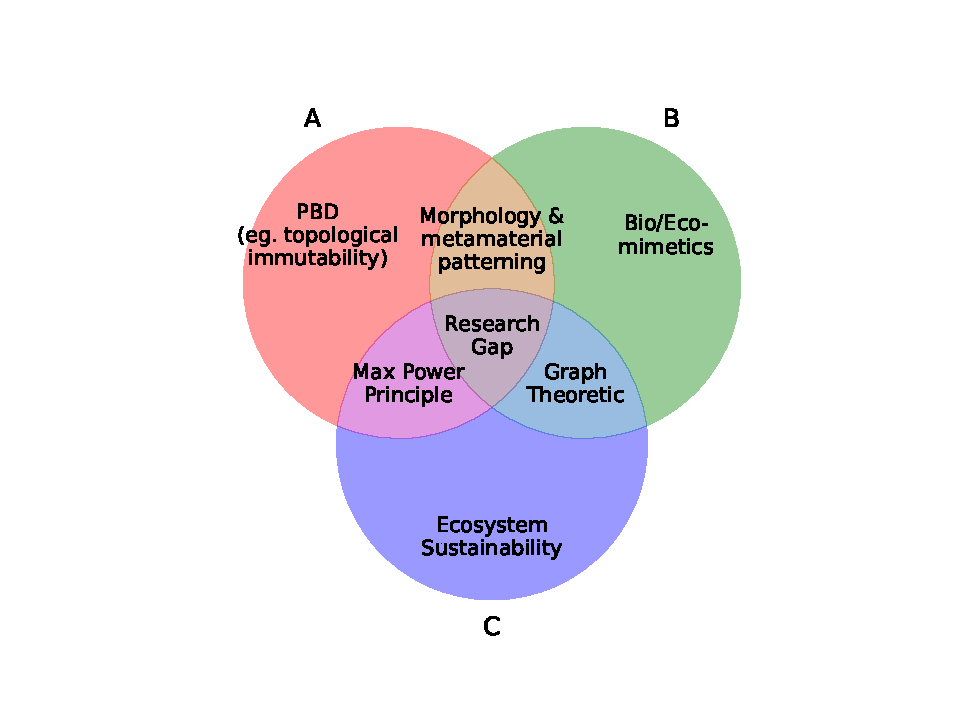
\includegraphics[width=0.7\linewidth]{ven}
    \caption{Venn chart of the interacting conceptual framework used in this thesis.}
    \label{fig:conceptual:framework}
\end{figure}

This review is Part B of a two part literature review. Part A introduced the conceptual framework given in the Introduction (reproduced in Fig.~\ref{fig:conceptual:framework} for convenience), and was concerned with the `Eco/Biomimetics' literature, the `Ecosystem Sustainability' literature and the overlap between these domains through the methods of ecological Graph Theoretics. The present chapter is concerned with the concept of `Principle' as a basis of `Principle Based Design' (PBD), that is the use of natural and geometric principles as a basis of design practice, and overlaps that PBD has with Ecosystem Sustainability and Eco/Biomimetics in the conceptual framework. Part B will begin by focusing on the \SE---an ancient water wheel for lifting water---as the primary design case which will be used to demonstrate PBD, and to explain the emergence of PBD in the early modern period through the works of \citeauthor{descartes_principles_1982}. After introducing the historical background to PBD and the \SE, the review will then consider contemporary work that has looked as waterwheel designs that are similar to the \SE.

% This introduction aims to answer questions of motivation: ``was is the \SE?'', ``why the \SE?'', ``why PBD?'' and ``why now?'' 

% Following this introduction the literature review is broken into two parts (A and B). Part A is historical and looks at the emergence and transformation of PBD. It uses the \SEs as the design case for facilitating answers the questions, ``what is PBD?'', and ``where did PBD come from?'' Part B considers the contemporary context and seeks to answer the question, ``who else is looking at this at the moment?'' in the context of modern digital fabrication techniques such as CAD and CAM systems. 

\section{History of \SE}
\label{sec:history:of}

\begin{quotation}
    ``Science mattered in a negative sense: Reynolds demonstrates that deficiencies of pre-19th-century wheels were clearly related to inadequate understanding of their principles of operation.'' \citep[p.827]{constant_review_1985}
\end{quotation}

This understanding, says \citeauthor{constant_review_1985}, was made possible in the late 18C with a convergence of problems of work and energy with hydraulic phenomena \citeyearpar[p.827]{constant_review_1985}. \citeauthor{constant_review_1985} does not elaborate on this comment, rather leaving us to refer back to an unnamed chapter in \citeauthor{reynolds_stronger_2002}'s book on the history of water wheels. 

Before we consider \citeauthor{reynolds_stronger_2002}'s work, it is my thesis that \citeauthor{constant_review_1985} has glossed over some important factors here. One factor is that the so-called ``problems of work and energy'' had arisen in one of the most famous disputes of the period, the `\textit{vis viva} dispute'. It was a dispute which had been between the supporters of Newton and Leibniz, but had also arisen out of Descartes'  natural philosophy and metaphysics.  

In \citeauthor{reynolds_stronger_2002}'s





\section{A brief introduction to PBD} 
\label{sec:what:pbd}

In brief terms, the idea of PBD motivating this thesis refers to \citeauthor{descartes_principles_1982}' treatment of natural and geometric principles (See Sec.~\ref{sec:cartesian:principle}). The interest here is to use Cartesian principles  developed in the early modern period (circa 1450 \CEs to 1750 \CE), together with modern derivations (circa 1750 \CEs onwards) to inform computational design practice. Part A of the literature review attempts give a more detailed account of this concept by tracing the development of \SEs, and the emergence of PBD in the early modern period with reference to the `re-design' of the \SEs. 

\citeauthor{descartes_principles_1982}' philosophy has itself had significant implications for contemporary design practice because, not only do we refer to Cartesian machines in reference to his Geometric system, but because some of his geometric principles also found their way in to CAD systems. However, it is his natural principles which appear to have been the cause of much confusion. But if this thesis is right his natural principles have had practical relevance to the definition of PBD, especially in relation to the design of water wheels in the century after \citeauthor{descartes_principles_1982}' death.

\section{What is a Cartesian principle?} 
\label{sec:cartesian:principle}

This section aims to introduce \citeauthor{descartes_principles_1982}' concept of `Principle'.\footnote{Since \citeauthor{descartes_principles_1982}' objective is to direct our attention towards the invariants of abstract mathematics and geometry I have omitted his theistic arguments which appeal to the immutability of a supreme perfect being, that is, God. The reasons for appealing to God here are complex, and in part aimed to justify the claim that there is some invariance this his Principles refer to exists. My reason for this omission is that I believe \citeauthor{descartes_principles_1982} may have been writing in a context whereby not only was there penalty for presenting ideas contrary to doctrine (as evidenced by the house arrest of Galileo), but he was also having to convince the clergy of the pedagogic value in attending to abstract mathematics and geomtry.} To do so it might be helpful to go back a step and consider why \citeauthor{descartes_principles_1982} thought they might be necessary; why is \citeauthor{descartes_principles_1982} talking about `Principles'? To answer this question we might first consider his \textit{Meditations} where \citeauthor{descartes_meditations_2013} engaged in a process known as \textit{radical doubt}. Since we can believe in falsehoods and be deceived by our senses, \citeauthor{descartes_meditations_2013}' \textit{radical doubt} questions all of his previous opinions. In the \textit{Meditations} he writes, ``I am here quite alone, and at last I will devote myself sincerely and without reservation to the general demolition of my opinions'' \citep[\S~18, p.~12]{descartes_meditations_2013}.

Against this background \citeauthor{descartes_principles_1982} viewed the practice of philosophy,\footnote{\citeauthor{descartes_principles_1982} called this pracitce, `the study of Wisdom' \citet[p.~xvii]{descartes_principles_1982}, or `philosophizing'.} as a method for removing this doubt by creating certainty and thereby perfecting our knowledge \citeyearpar[p.~xvii]{descartes_principles_1982}. \citeauthor{descartes_principles_1982} reckoned that such a method should  search for, and promote, ideas that qualify as `first causes', or `Principles' \citeyearpar[p.~xvii]{descartes_principles_1982}, proceeding on the `maxim' that we, ``\dots reject all such merely probable knowledge and make it a rule to trust only what is completely known and incapable of being doubted'' \citep[Rule~II,p.~3]{descartes_philosophical_1911}. And to qualify as principles, says \citeauthor{descartes_principles_1982}, our ideas must meet two conditions:

\begin{quotation}
    ``\dots first, they must be so clear and so evident that the human mind cannot doubt of their truth when it attentively considers them; and second, the knowledge of other things must depend upon these Principles in such a way that they may be known without the other things, but not vice versa.'' \citep[p.~xvii]{descartes_principles_1982}
\end{quotation}

To remove doubt \citeauthor{descartes_principles_1982}' goal is to direct our attention towards Arithmetic and Geometry, ``\dots that in our search for the direct road towards truth we should busy ourselves with no object about which we cannot attain a certitude equal to that of the demonstrations of Arithmetic and Geometry'' \citep[Rule~II,p.~5]{descartes_philosophical_1911}. \citeauthor{descartes_principles_1982} seems to have believed that Arithmetic and Geometry could provide us with a source of ideas that qualified as  Principles because they could remove our doubt and may be known without reference to other things. He begins with the example of a triangle whose theorems had been known to the Ancients:

\begin{quotation}
    ``For example, when I consider the nature of a triangle, it appears most evident to me, steeped as I am in the principles of geometry, that its three angles are equal to two right angles; and so long as I attend to the proof, l cannot but believe this to be true.'' \citep[p.~48, \S~40]{descartes_meditations_2013}
\end{quotation}

By attending to Arithmetic and Geometry, \citeauthor{descartes_principles_1982} hopes that we may conceive of immutable truths, that is, constancies and invariances, that exist independently of our thought. In other words, Principles are independent of our mind, but we cannot doubt them whenever we comprehend them:

\begin{quotation}
    ``For example, when I imagine a triangle, although there may nowhere in the world be such a figure outside my thought, or ever have been, there is nevertheless in this figure a certain determinate nature, form, or essence, which is immutable and eternal, which I have not invented, and which in no wise depends on my mind,'' \citep[p.~180]{descartes_philosophical_1911}
\end{quotation}

The Cartesian Principle has, then, a somewhat curious existence. Although it is immutable and eternal, and does not depend on our minds, since it does not exist outside our thought, it is only eternal so long as we conceive it, and yet it is the basis of forming certainty and true ideas. Moreover, although in contemporary terms we use terms like `physics envy' to refer to physics as the `superior science', for \citeauthor{descartes_principles_1982} we don't come to comprehend Principles through physics, rather we comprehend Principles in physics through Geometry and abstract Mathematics:

\begin{quotation}
    ``That I do not accept or desire in Physics any other principles than in Geometry or abstract Mathematics; because all the phenomena of nature are explained thereby, and certain demonstrations concerning them can be given.'' \citep[\S~64, p.~76]{descartes_principles_1982}
\end{quotation}

As he explains in \textit{The Principles} this is why he writes a book on Geometry as an annex to his \textit{Discourse on the Method of rightly conducting one's reason and seeking truth in the sciences}:

\begin{quotation}
    ``\dots in the Geometry, I sought to demonstrate that I had discovered many things which were previously unknown and thus to provide grounds for believing that many others can still be discovered, in order to thereby incite all men to the search for truth.'' \citep[p.~xxv]{descartes_principles_1982}    
\end{quotation}

But the seemingly curious existence of Cartesian Principles, can, it would seem, be clarified computationally. Indeed it is through computational examples that we might begin to understand what  \citeauthor{descartes_principles_1982} is referring to, so we will now look at a couple of examples.


% let us proceed to explain more carefully our reasons for saying, as we did a little while ago, that of all the sciences known as yet, Arithmetic and Geometry alone are free from any taint of falsity or uncertainty.








% \subsection{Ideas at any scale}
% \label{sub:sec:all:ideas}

% It is important to emphasise two considerations here. Firstly, and perhaps less controversially, is that \citeauthor{descartes_principles_1982} is talking about all possible knowledge. From his first condition above, \citeauthor{descartes_principles_1982} hopes that by seeking Principles we might generate clear and evident ideas whose truth cannot be doubted, and from them, ``\dots deduce the reasons for \textit{everything} which we are capable of knowing'' \citeyearpar[my emphasis, pp.~xvii,xix]{descartes_principles_1982}. His book on \textit{The Principles}, says \citeauthor{descartes_principles_1982}, contains:

% \begin{quotation}
%     ``\dots everything which is most general in Physics, namely, the explanation of the first laws or Principles of Nature, and the way in which the Heavens, the fixed Stars, the Planets, the Comets, and generally all the universe is composed.'' \citep[p.~xxv]{descartes_principles_1982}
% \end{quotation}

% It is an ambitious agenda. \citeauthor{descartes_principles_1982} is saying that any idea about anything, any substance, any system, at any scale, quantum or cosmic, can only be clear and evident if it based on a Principle or `first-cause', and by implication subject to the two conditions noted above. If we think about this in terms of PBD, it would mean that the same design Principles might be applied at all scales of design. Whether it is the design of a quantum switch, or the design of a retail product, a building, a landscape, an economy or a planetary system like a Mars colony, the same Principles will apply. But how they might be applied is a little unclear, and indeed one aim of this thesis is to seek a clarification. 

% The modern tradition that might have the closest match to \citeauthor{descartes_principles_1982}' agenda here is the General Systems Theory (GST) of \citeauthor{bertalanffy_general_1969}.\footnote{See \citet{bertalanffy_theory_1950,bertalanffy_problems_1951,bertalanffy_general_1969,bertalanffy_unity_1973,bertalanffy_outline_2008}.} \citeauthor{bertalanffy_general_1969} traced the origins of GST to the early modern Enlightenment philosophy of W.G.v.Leibniz,\footnote{\citeauthor{bertalanffy_general_1969} traced the origins of GST and the `systematic spirit' of GST back through thinkers like Marx and Engles, Vico and ibn Kaldun, Paracelsus and Nicholas of Cusa. In Section~\ref{sec:leibniz:env:eng} we will will look at the precursors to Leibniz writing in more detail, but needless to say, some of \citeauthor{leibniz_gottfried_1970}'s ideas were developed in response to \citeauthor{descartes_principles_1982}.} but he identified Lotka\footnote{\citet{lotka_contribution_1909,lotka_objective_1914,lotka_efficiency_1915,lotka_analytical_1920,lotka_note_1921, lotka_contribution_1922,lotka_natural_1922,lotka_two_1924,lotka_contribution_1939,lotka_law_1945,lotka_elements_1957}.} as the person who came closest to elaborating the formal foundations of GST which aimed to give, ``\dots the most general properties of inorganic compared to organic systems'' \citep[p.~11]{bertalanffy_general_1969}. In the context of computational design, \citeauthor{descartes_principles_1982}' agenda was discussed by \citeauthor{menges_computational_2011}. \citeauthor{menges_computational_2011} considered GST to be a new scientific discipline whose subject matter was the , ``\dots formulation of principles that are valid for `systems' in general, whatever the nature of their component elements and relations or `forces' between them'' \citep[p.~51]{menges_computational_2011}. Indeed from this perspective, the subject matter of GST appears to have the same goals as \citeauthor{descartes_principles_1982}' \textit{Principles of Philosophy}, such that, to paraprhase \citeauthor{descartes_principles_1982} and \citeauthor{menges_computational_2011}, the formulation of principles that are valid for systems in general will enable us to deduce the reasons for everything which we are capable of knowing.

% \citeauthor{menges_computational_2011} identify two critical conditions of GST that are relevant to the next section which addresses \citeauthor{descartes_principles_1982} concept of causation, so they will be mentioned here briefly. These are, \textit{equifinity}  and \textit{feedback}. The word `equifinity' here refers to a dynamic and functioning steady state of a system which can be achieved from various starting points \citep[p.~50]{menges_computational_2011}. `Feedback' refers to information which specifies actions and transformations required for a system to reach a functioning steady state \citep[p.~50]{menges_computational_2011}. And it is the idea of feedback information that specifies the transformations required to reach equifinity that is relevant to   \citeauthor{descartes_principles_1982}' concept of causation to which we now turn. 

% \subsection{Cartesian causation}
% \label{sub:sec:cartesian:causation}

% A second consideration is perhaps the most contentious. It is not something that this thesis aims to resolve, however a viewpoint will be offered.\footnote{This viewpoint does not seek to advocate any forms of theism, atheism or agnosticism. Rather the aim is to provide a mechanism by which we may develop a clearer idea of Cartesian Principles.} With reference to the two critical conditions of GST identified by \citeauthor{menges_computational_2011}, \citeauthor{descartes_principles_1982}' causation and the intended outcome of the concept might be considered as equifinite, such that we can arrive an an appreciation of it from two different starting points. These starting points might be considered as two different cohorts, or human populations; a theist cohort, and  a cohort of atheists or agnostics. Although the second cohort was heretic at the time (with Galileo famously under house arrest), it seems that he has devices for both so that he could establish the concepts of Principle.

% For the first cohort, \citeauthor{descartes_principles_1982}' idea of causation refers to the, `first-cause', which he also exchanges with the word, `Principle'. In this concept of causation, the `first-cause', appears to be bound to the ideas of both `motion' and an `effect',\footnote{I quote these terms because they have been the source of considerable debate and investigation in the History and Philosophy of Engineering Science.} that is, movement, or a change in direction or speed, an action in time, and an action over time. He is concerned to set up a circumstances whereby we can conceive of constancy amidst any changes, and percieve invariance in dynamic environments. 





% we might concieve of a supremely perfect being as exitentially equifinite, always existing in the same, unchanging, constant, immutable steady functional state, whereby, at a cosmic scale, this exitential equifinity amounts to a goal function whose causal objective is to maintain a constant quantity of motion. 




% Whilst a motion generated by some cause seems to make the world around us appear mutable and constantly transforming through growth, decay and innovation, how can there be something that is immutable and unchanging?  \citeauthor{descartes_principles_1982} answers this with an appeal to theism, that is, the belief in the existence of a God who intervenes in the universe. Hence \citeauthor{descartes_principles_1982} wants to encourge the following view: 

% \begin{quotation}
%     ``That God is the primary cause of motion; and that He always maintains an equal quantity of it in the universe'' \citep[\S~36, p.~57]{descartes_principles_1982}
% \end{quotation}

% In my view, this statement is \citeauthor{descartes_principles_1982}' linguistic device that has the intended outcome of establishing the acceptability of the concepts of immutability, or constancy which we aims to locate as central notions involved with the concept of `Principle'. In other words, a `Principle' refers to something that remains immutabile, constant, or invariant under changing conditions. To consolodate this idea he appeals to one of the most General ideas that the theistic cohort is willing to accept. That is the idea of a supremely perfect being, whose perfection is expressed by their immutability. If a supremely perfect being is the primary or first-cause, their action simultaneously brought about motion and Principles of motion such that an expression of the supreme being's perfection is their immutability, and that immutability is the Principle that equal, constant quantity of motion is conserved in the universe. This is \citeauthor{descartes_principles_1982} causal model. The first-cause at one in the same time generates motion, and generates a Principle that refers to conservation of motion, the latter of which is more familiar to modern thinking as `the first Law', which appears in thermodynamics and energetics as the conservation of energy, and also as the conservation of mass.

% So long as there is a cohort that believes in a supremely perfect being whose perfection is expressed by their constant action, \citeauthor{descartes_principles_1982} seems to have thought that his metaphysics was on a good footing. For the theist, \citeauthor{descartes_principles_1982} appeals to this exitentially immutable first-cause, the invariant nature of a supremely perfect being, as a way out of radical doubt. 

% ``Finally, if there be still persons who are not sufficiently persuaded of the existence of God and of the soul, by the reasons I have adduced, I am desirous that they should know that all the other proposi tions, of the truth of which they deem themselves  ''

% But this appeal to the theistic cohort, as I suggested above, may not appeal to contemporary atheists or agnostics, hence possibly leaving them in the state of radical doubt and doubting the existance of \citeauthor{descartes_principles_1982}' concept of any Principles. For this cohort, \citeauthor{descartes_principles_1982} also appears to have a second strategy for which it is not necessary to appeal to the belief in a supremely perfect being. That we can doubt is the key to this second strategy. To borrow from the famous phrase, `I think therefore I am', we might consider the first principles as more, `I doubt therefore I am':

% \begin{quotation}
%     ``Thus, considering that he who wishes to doubt everything nevertheless cannot doubt that he exists while he is doubting, and that what reasons thus (being unable to doubt itself and yet doubting all the rest) \dots'' \citep[p.~xxi]{descartes_principles_1982}
% \end{quotation}

% The undoubtable existence of a doubting person is \citeauthor{descartes_principles_1982}' way out of radical doubt for the second cohort. But for this cohort he still seeks a way of introducing the concept of Principle.  



% It is incorporeal, metaphysical, and is something that we believe irrespective of verification. It is unfalsifiable. 

% The maintenance of an equal quantity of motion is an instantiation of the exitentially immutable nature of a supremely perfect being \citep[\S~15, pp.~9-10]{descartes_principles_1982}, by which he means God. 




% % The human mind, ``\dots will understand that this idea of a supremely perfect being has not been devised by it'' \citep[\S~15, pp.~9-10]{descartes_principles_1982} \dots a true and immutable nature, and one which cannot fail to exist; since necessary existence is contained within it''

% \subsection{\citeauthor{descartes_principles_1982}' method}

% How, then, can we go about developing ideas that contain a truth that cannot be doubted and identifying such as Principles? What was a Cartesian `Principle'? From the treatment above is it something immutable, unchanging even when the physical environment or the thing itself is changing and transforming? So how then, do we identify this immutability? For \citeauthor{descartes_principles_1982} we can begin to comprehend these invariances not through physics, but through Geometry and abstract Mathematics:

% \begin{quotation}
%     ``That I do not accept or desire in Physics any other principles than in Geometry or abstract Mathematics; because all the phenomena of nature are explained thereby, and certain demonstrations concerning them can be given.'' \citep[\S~64, p.~76]{descartes_principles_1982}
% \end{quotation}

% For both cohorts, theists and the atheisits \& agnostics, we can begin to see the principles through the study of Geometry and abstract Mathematics. As he explains in \textit{The Principles} this is why he writes a book on Geometry as an annex to his \textit{Discourse on the Method of rightly conducting one's reason and seeking truth in the sciences}:

% \begin{quotation}
%     ``\dots in the Geometry, I sought to demonstrate that I had discovered many things which were previously unknown and thus to provide grounds for believing that many others can still be discovered, in order to thereby incite all men to the search for truth.'' \citep[p.~xxv]{descartes_principles_1982}    
% \end{quotation}

\section{Introductory examples}
\label{sec:examples}

Three introductory examples of Principles will be considered here to demonstrate the kind of constancy or invariance that, if this thesis is right, \citeauthor{descartes_principles_1982} was intending us to perceive. The key here is that the invariance can be deomstrated accross several transformations of a shape. But firstly a note on the nomenclature that \citeauthor{descartes_philosophical_1911} introduces. He writes,  ``\dots we shall employ the characters a, b, c, etc. for expressing magnitudes already known, and A, B, C, etc. for symbolising those that are unknown'' \citep[Rule~XVI, p.~67]{descartes_philosophical_1911}. This is important to note for several reasons. Firstly it amounts to \citeauthor{descartes_philosophical_1911}' introduction of algorithmic geometry, and he is doing so for the purpose of reducing load on memory, and thereby placing an emphasis on generality rather than specific numbers.  

\subsection{Triangles: XYZ' Theorem}
\label{subsec:triangles}

% A note on nomenclature here, `Theorem' is a mathematical instatiation of a Principle. 

\citeauthor{descartes_philosophical_1911} gives us a right-angled triangle whose adjacent side has a value of 12, and opposite side is 9, and he poses the problem of finding the length of the hypotenuse from these two parameters. His intent is to show and contrast his new method of algorithmic geometry with the method of the Arithmeticians, ``\dots if we are trying to find the hypotenuse of the right-angled triangle whose sides are 9 and 12, the Arithmetician will tell us that it is \(\sqrt{225}\), i.e. 15 '' \citeyearpar[Rule~XVI, p.~67]{descartes_philosophical_1911}.\footnote{\citeauthor{descartes_philosophical_1911} doesn't think much of Arithmetic methods writing, ``\dots with Arithmeticians, who, if the result required turns up, are quite content even though they do not perceive how it depends upon the data, though it is really in knowledge of this kind alone that science properly consists.'' \citeyearpar[Rule~XVI, p.~69]{descartes_philosophical_1911}.} A reproduction of \citeauthor{descartes_philosophical_1911}' triangle is given in figure~\ref{fig:triangle:91215} for reference. Here \citeauthor{descartes_philosophical_1911} uses the capitalised symbols ABC because, in this example, the magnitudes of the \(x,y\) and \(z\) co-ordinates for the vertices is unknown:\footnote{Even though this is only a 2D depiction, whilst all z co-ordinates are the same, the magnitude is nevertheless unknown.} 
 
\begin{figure}[ht!]
    \centering
    \includegraphics[width=0.35\linewidth]{1911_descartes_ABCtriangle_p69}
    \caption{\citeauthor{descartes_philosophical_1911} example of a right-angled triangle \citeyearpar[p.~69]{descartes_philosophical_1911}}
    \label{fig:triangle:91215}
\end{figure}

Now lets take several different versions of the triangle shown in figure~\ref{fig:triangle:91215} to demonstrate the problem with the Arithmetic method that \citeauthor{descartes_philosophical_1911} is pointing to. Consider figures~\ref{fig:triangle:345}-\ref{fig:triangle:51213} and Table~\ref{tab:arithmetic}:


\begin{figure}[ht!]
    \centering
    \subfloat[]{
        % \resizebox{.75\linewidth}{!}{ 
            \begin{tikzpicture}[every node/.style={scale=.75}] %[scale=.45\linewidth]
                \coordinate [label=left:B] (B) at (0,0);
                \coordinate [label=left:A] (A) at (0,3*\triadj);
                \coordinate [label=right:C] (C) at (4*\triadj,0);
                \draw (C) -- node[below] {$4$} (B) -- node[left] {$3$} (A) -- node[above] {$5$} (C);
                \draw (0,0) rectangle (1*\triadj,1*\triadj);
                \tkzMarkAngle[size=1*\triadj,color=cyan,mark=|](A,C,B)
                \tkzMarkAngle[size=1*\triadj,color=cyan,mark=|](C,B,A)
            \end{tikzpicture}
            \label{fig:triangle:345}
        % } sxm108.adm
    }
    \subfloat[]{
        % \resizebox{.75\linewidth}{!}{ 
            \begin{tikzpicture}[every node/.style={scale=.75}]  %[scale=.45\linewidth]
                \coordinate [label=left:B] (B) at (0,0);
                \coordinate [label=left:A] (A) at (0,6*\triadj);
                \coordinate [label=right:C] (C) at (8*\triadj,0);
                \draw (C) -- node[below] {$8$} (B) -- node[left] {$6$} (A) -- node[above] {$10$} (C);
                \draw (0,0) rectangle (1*\triadj,1*\triadj);
                \tkzMarkAngle[size=1*\triadj,color=cyan,mark=|](A,C,B)
                \tkzMarkAngle[size=1*\triadj,color=cyan,mark=|](C,B,A)
            \end{tikzpicture}
            \label{fig:triangle:6810}
        % }
    }
    \subfloat[]{
        % \resizebox{.75\linewidth}{!}{ 
            \begin{tikzpicture}[every node/.style={scale=.75}]  %[scale=.45\linewidth]
                \coordinate [label=left:B] (B) at (0,0);
                \coordinate [label=left:A] (A) at (0,5*\triadj);
                \coordinate [label=right:C] (C) at (12*\triadj,0);
                \draw (C) -- node[below] {$12$} (B) -- node[left] {$5$} (A) -- node[above] {$13$} (C);
                \draw (0,0) rectangle (1*\triadj,1*\triadj);
                \tkzMarkAngle[size=1*\triadj,color=cyan,mark=|](A,C,B)
                \tkzMarkAngle[size=1*\triadj,color=cyan,mark=|](C,B,A)
            \end{tikzpicture}
            \label{fig:triangle:51213}
        % }
    }
    \caption{More different right-angled triangles.}
    \label{fig:triangles:theorems}
\end{figure}



\begin{table}[h!]
    \small 
    \centering
    \begin{tabular}{lccr} 
        Fig. & Opp. & Adj. & Hypotenuse \\
        \hline
        \ref{fig:triangle:345}) & 3 & 4 & \(\sqrt{25}\) = 5 \\	
        \ref{fig:triangle:6810}) & 6 & 8 & \(\sqrt{100}\) = 10  \\	
        \ref{fig:triangle:51213}) & 5 & 12 & \(\sqrt{169}\) = 13 \\	
        \ref{fig:triangle:91215}) & 9 & 12 & \(\sqrt{225}\) = 15  \\	    
    \end{tabular}
    \caption{Arithmetic method for calculating hypotenuse.}
    \label{tab:arithmetic}
\end{table}

Table~\ref{tab:arithmetic} shows the different calculations using an Arithmetic method. But by tabluating the calculations in this eay, it is (at least to me) difficult to percieve any invarience, because there is nothing constant accross the different calcuations. This is to say that, although the method is the same, the numbers and results are always different for different sized triangles: 

% \begin{quotation}
%     ``\dots while Arithmeticians have been wont to designate undivided magnitudes by groups of units, or else by some number, we on the other hand abstract at this point from numbers themselves no less than from Geometrical figures or anything else, as we did a little time ago. Our reason for doing this is partly to avoid the tedium of a long and superfluous calculation, but chiefly that those portions of the matter considered which are relevant to the problem may always remain distinct, and may not be entangled with numbers that are of no help to us at all.'' \citeyearpar[p.~67]{descartes_philosophical_1911}
% \end{quotation}



But instead of using an Arithmetic method, \citeauthor{descartes_philosophical_1911} uses the nomenclature above and says, ``\dots we shall write a and b in place of 9 and 12, and shall find the hypotenuse to be \(\sqrt{a^2 + b^2}\)  '' \citeyearpar[Rule~XVI, pp.~67-68]{descartes_philosophical_1911}. 
, but also because he is seeking to state the problem abstractly so he can show a general method for deriving hypotenuse length from the lengths of the sides \citeyearpar[Rule~XVI, pp.~69-70]{descartes_philosophical_1911}

% \begin{tikzpicture}[scale=.1]


\begin{figure}[ht!]
    \centering
    \subfloat[Specific parameter values]{
        \centering
        \includegraphics[width=0.35\linewidth]{1911_descartes_ABCtriangle_p69}
        % \resizebox{.5\linewidth}{!}{ 
            % \begin{tikzpicture} %[scale=1.2]
            %     \coordinate [label=left:B] (B) at (0,0);
            %     \coordinate [label=left:A] (A) at (0,9*\dualadj);
            %     \coordinate [label=right:C] (C) at (12*\dualadj,0);
            %     \draw (C) -- node[below] {$12$} (B) -- node[left] {$9$} (A) -- node[above] {$15$} (C);
            %     \draw (0,0) rectangle (1,1);
            %     \tkzMarkAngle[size=1*\dualadj,color=cyan,mark=|](A,C,B)
            %     \tkzMarkAngle[size=1*\dualadj,color=cyan,mark=|](C,B,A)
            % \end{tikzpicture}
        % }
        % \label{fig:triangle:91215}
    }
    \subfloat[Generalised parameters]{
        % \resizebox{.75\linewidth}{!}{ 
            \begin{tikzpicture} %[scale=.45\linewidth]
                \coordinate [label=left:B] (B) at (0,0);
                \coordinate [label=left:A] (A) at (0,9*\dualadj);
                \coordinate [label=right:C] (C) at (12*\dualadj,0);
                \draw (C) -- node[below] {B} (B) -- node[left] {A} (A) -- node[above] {C} (C);
                \draw (0,0) rectangle (1*\dualadj,1*\dualadj);
                \tkzMarkAngle[size=1*\dualadj,color=cyan,mark=|](A,C,B)
                \tkzMarkAngle[size=1*\dualadj,color=cyan,mark=|](C,B,A)
            \end{tikzpicture}
        % }
    }
    \caption{LHS image from \citet[p.~69]{descartes_philosophical_1911}. RHS image a depiction of \citeauthor{descartes_philosophical_1911}' algebraic geometry.}
    \label{fig:triangles:theorems}
\end{figure}


His goal is to afford us the perception that: 

\begin{quotation}
    ``\dots a hypotenuse whose length is 15 is commensurable with sides whose lengths are 9 and 12, quite apart from the general law that it is the hypotenuse of a right-angled triangle whose sides are as 3 to 4.'' \citep[Rule~XVI, p.~69]{descartes_philosophical_1911}
\end{quotation}


invariance in all ABC right-angled triangles.

\begin{table}[h!]
    \small 
    \centering
    \begin{tabular}{cccc} 
        \textit{a} & \textit{b} & \(\sqrt{a^2 + b^2}\) & c \\
        \hline
        9 & 12 & \(\sqrt{9^2 + 12^2}\) & 15 \\	
        3 & 4 & \(\sqrt{3^2 + 4^2}\) & 5 \\	
        
        \hline
    \end{tabular}
    \caption{\textit{Invariance}.}
    \label{tab:algebraic}
\end{table}


\subsection{Circles: XYZ' Theorem}
\label{subsec:circle}

The second example is another one that was familiar to the ancients, \(\pi\). No matter how we change the radius of a circle, \(\pi\), the ratio of circumference to diameter, remains constant.



\subsection{Topological immutability: \citeauthor{descartes_principles_1982}' Theorem}
\label{subsec:topological:immutability}

The final example here comes from \citeauthor{descartes_principles_1982} himself. 

These Principles referred to constancies amidst change that could be identified and used as the basis of this indubitable epistemology,\footnote{
This phrase is echoed by \citeauthor{lindsay_energy_1975} \citeyearpar[p.5]{lindsay_energy_1975} who discussed quantities that remained constant in the midst of change. It is also the kind of invariance that is characteristic of \citeauthor{gibson_ecological_1986} ecological perception, invariance \citeauthor{gibson_ecological_1986}'s ecological psychology puts emphasis on the perception of invariance in dynamic environments. The specific invariance of interest in the present work is the parameter of river flow. \citeauthor{gibson_ecological_1986}'s focus on perception of invariance.} and the first constancy, the first cause or principle, 



The constancy that \citeauthor{descartes_principles_1982} is pointing to here as his first principle is our faculty to doubt everything at all time. This faculty to doubt is a constant, and from this beginning \citeauthor{descartes_principles_1982} then appeals to an all-knowing God as the source of all truth, and which enables us to perceive principles. But the principles he starts with concern, ``immaterial or Metaphysical things'' \citeyearpar[p.~xxii]{descartes_principles_1982}. From those Principles he then proceeds to, ``\dots very clearly deduce the Principles of corporeal or Physical things; namely that there are bodies extended in length, width, and depth, which have diverse figures and are moved in diverse ways'' \citeyearpar[p.~xxii]{descartes_principles_1982}. 

For corporeal things he says, 

``That is, an object's motion can be altered only by the impact of another body. In a letter to de Beaune, written in April, 1639, Descartes states: `\dots all my Physics is merely Mechanics \dots'; A. \& T., II, 541-544.'' \citep[Miller and Miller in Fn.~14, p.~52]{descartes_principles_1982}


By starting with immaterial or Metaphysical principles, \citeauthor{descartes_principles_1982} thought that truth in one's ideas did not have to refer to any physical domain of knowledge, like physics or mechanics since \citep[p.~xvii]{descartes_principles_1982}. Rather one only needed geometry and mathematics. This clarity and certainty could be established through the study of Geometry and abstract Mathematics \citep[Part~II, Principle~64, p.~76]{descartes_principles_1982}. This was because Geometry and abstract Mathematics could enable a conception of principles based on regularities, invariants and constancy evident in form and motion. 

A classic example of such invariance, which was worked out well before \citeauthor{descartes_principles_1982}' time is \(\pi\). No matter how we change the radius of a circle, \(\pi\), the ratio of circumference to diameter, remains constant. 

\citeauthor{descartes_principles_1982}' further addition to the geometric principles was what is referred to as \textit{topological invariance}. This discovery has been attributed to Euler, however more recent scholarship and translation of Leibniz's notes have attributed it to \citeauthor{descartes_principles_1982}.\footnote{See \citeauthor{aczel_descartess_2006}'s intriguing story \citep[pp.~225-228]{aczel_descartess_2006}.} Today it is commonly called Euler's theorem, however for the pupose of the narrative presented here I will refer to it as \citeauthor{descartes_principles_1982}' theorem. The geometric principle specified in \citeauthor{descartes_principles_1982}' theorem is found in Platonic solids and is expressed in the relation of face, vertices and edge. Figure~\ref{fig:topological} shows these elements using colour-coding to establish the association between the words and the geometric characteristics. Hence we might specify \citeauthor{descartes_principles_1982}' theorem as, \textcolor{aliceblue}{\textit{faces}} + \textcolor{cyan}{\textit{vertices}} - \textcolor{red}{\textit{edges}}, and perform the calculation as shown in Steps \ref{eqn:theorem}-\ref{eqn:result} for the pyramid shown in Figure~\ref{fig:topological}:

% \begin{pycode}
% from matplotlib import pyplot as plt
% from mpl_toolkits.mplot3d.art3d import Poly3DCollection, Line3DCollection
% import numpy as np

% fig = plt.figure()
% ax = fig.add_subplot(111, projection='3d')

% # vertices of a pyramid
% v = np.array([[0, 0, 0], [1, 0, 0], [1, 1, 0],  [0, 1, 0], [0.5, 0.5, 1]])

% # generate list of sides' polygons of our pyramid
% verts = [ [v[0],v[1],v[4]], [v[0],v[3],v[4]], [v[2],v[1],v[4]], [v[2],v[3],v[4]], [v[0],v[1],v[2],v[3]]]

% # plot sides
% ax.add_collection3d(Poly3DCollection(verts, 
%  facecolors='cyan', linewidths=.5, edgecolors='r', alpha=.25))

% ax.scatter3D(v[:, 0], v[:, 1], v[:, 2])

% # ax.add_collection3d(Line3DCollection(verts, colors='k', linewidths=2))

% fig.savefig('topological.pdf')

% \end{pycode}

\begin{figure}[!h]
    \centering
    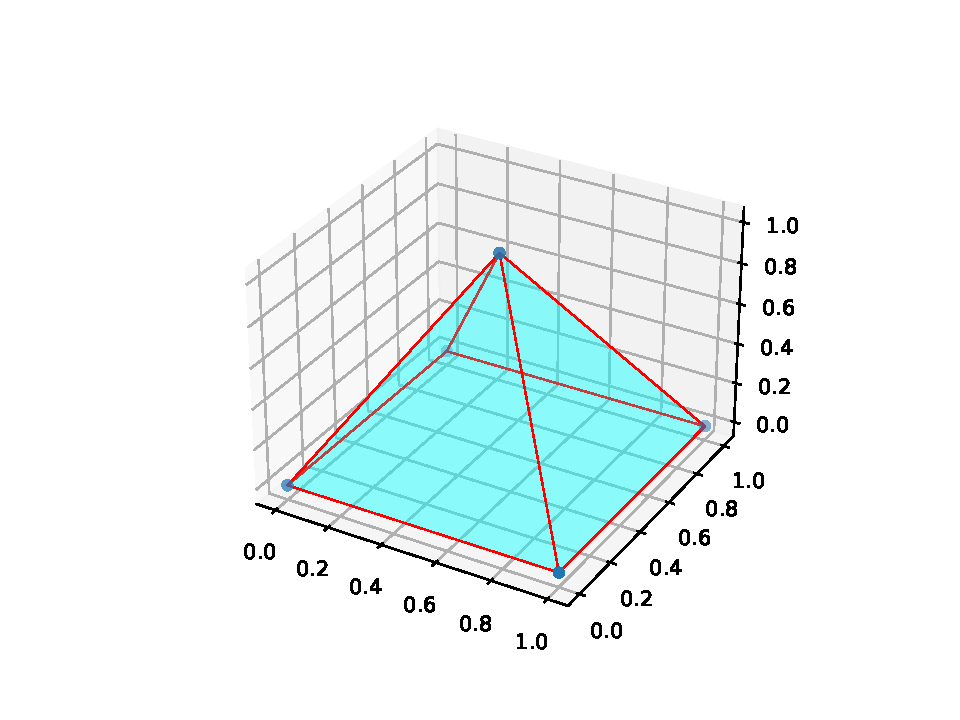
\includegraphics[width=0.8\linewidth]{topological}
    \caption{\textcolor{aliceblue}{\textit{Faces}}, \textcolor{cyan}{\textit{vertices}} and \textcolor{red}{\textit{edges}} of a pyramid.}
    \label{fig:topological}
\end{figure}

\begin{align}
    \text{Topological invariance} & = \textcolor{aliceblue}{\textit{faces}} + \textcolor{cyan}{\textit{vertices}} - \textcolor{red}{\textit{edges}}  && \textit{(Descartes' theorem)} \label{eqn:theorem} \\
    & = 5 + 5 - 8 \label{eqn:calc} \\
    & = 2  \label{eqn:result}
\end{align}

Steps \ref{eqn:theorem}-\ref{eqn:result} show the calculation which does not rely on the value for any particular parameter. The length of an edge, for example, can be transformed to any value, but the result for the calculation of \citeauthor{descartes_principles_1982}' theorem does not vary, and this constancy applies for other geometric forms like those shown in Table~\ref{tab:topological}, and thereby qualifies as a Cartesian geometric principle:

\begin{table}[h!]
    \small 
    \centering
    \begin{tabular}{lcccr} 
        \textbf{Platonic solid} & \textcolor{aliceblue}{\textbf{Faces}} & \textcolor{cyan}{\textbf{Vertices}} & \textcolor{red}{\textbf{Edges}} & \textbf{\citeauthor{descartes_principles_1982}' theorem} \\
        \hline
        Tetrahedron & 4 & 4 & 6 & \(4 + 4 - 6 =  2 \)  \\	
        Cube & 6 & 8 & 12 & \(6 + 8 - 12 =  2 \)  \\	
        Octahedron & 8 & 6 & 12 & \(8 + 6 - 12 =  2 \)  \\	
        Dodecahedron & 12 & 20 & 30 & \(12 + 20 - 30 =  2 \)  \\	
        Icosahedron & 20 & 12 & 30 & \(20 + 12 - 30 =  2 \)   \\
        \hline
    \end{tabular}
    \caption{\textit{Topological invariance} of Platonic solids.}
    \label{tab:topological}
\end{table}

\citeauthor{descartes_principles_1982}' take-home idea here is to encourage us to consider all the possible relationships between geometric parameters. Our goal is to seek equations for these relationships whose calculation always generates the same result, like \citeauthor{descartes_principles_1982}' theorem does. Such an equation, whose result remains constant under changing conditions, might then be call a theorem. But although the treatment above might produce geometric and mathematically interesting results, where we arrive at indubitable truths, that is, clear and distinct ideas without reference to any physical domain of knowledge, what happens when we want to practice natural philosophy and refer to a physical domain? We have established the idea of a geometric principle which might inform design practice, but what happened to the idea of a natural principle? What then is a natural principle, and how is it different to a geometric one?


Linear to angular velocity. 
\citet[p.764]{jablokow_topological_1993}

\section{Why the \SE?} 
\label{sec:why:se}

To my way of thinking the \SEs is a good design case to use in developing the narrative about the emergence of PBD in Part A of the literature review, because it is a relatively simple device that was used before and after PBD. Moreover, its design is amenable to the rapid iterative fabrication of modern digital methods. It is hoped, then, that the fabrication of \SEs can play a pedagogic role, and help us understand the idea of a principle and how natural principles in particular have relevance to design. Furthermore, \SEs design appears to have been directly transformed as a result of the changing ideas about design encapsulated in PBD. The \SEs artefact therefore gives us a level of continuity that is rare, and can show the evolution of design thinking over a relatively large timespan. Over this timespan the many varieties of water wheels, of which the \SEs is but one type, have had significant roles to play not just in the development of design and engineering science, but also in the history of the industrial revolution and the subsequent large-scale transformations of our environment, landscapes and societies. 

\section{Why PBD?} 
\label{sec:why:pbd}

definition of terms - why they are important to me

wheel as historical case study

Biomimic doesn't use geometric or natural principles 

Achim Menges

computational design thinking 




There are two main motivations for the focus on PBD. One is historical, connected to the reception of \citeauthor{descartes_principles_1982}' \textit{natural} principles in the transition from the early modern to the modern period. Another has a different historical thread, but has contemporary interest in what will be referred to here as `General and Ecological Systems Theory' (GEST).\footnote{\citet[p.~430]{odum_limits_1963} also used the term `general ecosystem theory'. `GEST' is used here to refer to the  significant work titled \textit{Ecological and General Systems} by \citet{odum_ecological_1994}. But it also aims to refer to the subsequent scholarship inspired by \citeauthor{odum_ecological_1994}'s approach (See \citet{hall_maximum_1995} for a review of subsequent schools of thought).} The GEST scholarship has attempted to integrate principles into the design of what they call ecological systems or `ecosystems'. 

The issue here is that whilst desaguliers noted the benefit, and whilst GEST believe there is benefit to using principels in sustainability, there is no clear method for PBD in either the literature arising in response to D's natural principels, or the GEST literature.  

Whilst \citeauthor{descartes_principles_1982}' \textit{geometric} principles progressed mathematics and are amenable to contemporary CAD technology, in the transition from the early modern to modern period \citeauthor{descartes_principles_1982}' \textit{natural} principles generated significant controversy and confusion. Indeed, contemporary scholarship still remains conflicted on the interpretation of \citeauthor{descartes_principles_1982}' natural principles, some scholars say that \citeauthor{descartes_principles_1982} was hopelessly wrong, others dispute the equations that scholars have used to quantify \citeauthor{descartes_principles_1982} principles. Either way, the contemporary disagreements have made it difficult to trace the relevance of \citeauthor{descartes_principles_1982}' natural principles to historical and contemporary design practice. 

The thesis is concrned to seek further clarification, and if 

In turn, the confusions that \citeauthor{descartes_principles_1982}' natural principles generated in the early modern period also led to the \textit{vis viva} disputes just after \citeauthor{descartes_principles_1982}' death. Again the \textit{vis viva} disputes have occupied much recent scholarship in the History and Philosophy of Engineering Science.\footnote{Although there is a significant amount of literature in the history and philosophy of science that is concerned with this dispute it remains unsettled with new views still emerging. See for example; \citet{hankins_eighteenth-century_1965, cardwell_factors_1967, iltis_controversy_1967, iltis_alembert_1970, iltis_leibniz_1971, iltis_leibnizian-newtonian_1973, gale_leibniz_1973, laudan_vis_1968-4, smith_vis_2006, hepburn_euler_2010, shimony_leibniz_2010a, reichenberger_leibnizs_2012, morris_john_2018-1}.} Circa 1730 the experimental philosopher \citeauthor{desaguliers_course_1734} called the confusion a kind of mechanical paradox. A paradox whereby, ``\dots a Power, whose Intensity is continually diminishing, does yet produce an Effect continually increasing'' \citeyearpar[my edit, p.~454]{desaguliers_course_1734}, such that ``\dots what is thus gained in Force by the Power, is lost in Time'' \citep[my edit, p.~518]{desaguliers_course_1734}. It is my contention that PBD can not only provide some insight into this confusion and the subsequent disputes, but also may have  as a response to this confusion. That is, PBD was used as a means of resolving the confusion, but also as a means of providing \textit{a priori} insight into design utility. However, PBD methods are poorly documented, and it is the precise specification of PBD which is the interest of this thesis---so that we can use PBD to resolve similar confusions in contemporary sustainable systems design. 

\section{What was the confusion, the value, and why now?} 
\label{sec:how:confusion}

In general terms the confusion seems to have been, and still is, located in our understanding of the relationship between environment and design. It is a relationship that is the subject of what \citeauthor{busbea_responsive_2019} \citeyearpar{busbea_responsive_2019} called the `environmental research manifold' (`the manifold') to analyse the rise of ecological psychology circa 1960. With a focus on the relations between environment and design, the research manifold speaks to contemporary concerns about environmentally sustainable design. Indeed, based on the climatic modelling reported by the IPCC, it is this manifold which appears to be presenting humanity with an epoch defining point-of-no-return in our history. Hence, the confusion surrounding PBD, and the potential that its clarification can help us create sustainable environment-design relations, provides an extra motivation to address these issues now. And if the thesis is right, the confusion first resided both in the definition of words, and in the environmental research manifold where wheel design parameters (wheel circumference etc.) were related to environmental factors like river flow.

In the transition from early modern to the modern period a `redesign' of water wheels like the \SE occurred. And the redesign was undertaken by using natural principles to guide the design process. For those that used the technique it also appears to have removed the prevailing confusion, and at that time, instrument makers like \citeauthor{smeaton_experimental_1759} (1724-1792CE) used scale models of water wheels (and windmills) as demonstrative aids to show both where the confusion arose and how to resolve it. So one outcome of the thesis is to reproduce \citeauthor{smeaton_experimental_1759} models with modern digital fabrication and rapid prototyping techniques to show how the experimental philosophers clarified the confusion and at the same time demonstrated the utility of PBD.

In the historical literature, the value of the approach was documented circa 1730 by the experimental philosopher \citeauthor{desaguliers_course_1734}. Moreover, \citeauthor{desaguliers_course_1734} argued that the absence of principles in design was likely to lead to the mismanagement of power systems like water wheels. This is the same narrative presented in this thesis; without PBD poor design outcomes occur when compared to PBD approaches. \citeauthor{desaguliers_course_1734} documented such an outcome by comparing the water wheels at the Gardens of Versailles in France (known as the `Engine at Marly'), with the water wheels at London Bridge. \citeauthor{desaguliers_course_1734} observed that the wheels in London, whose design was informed by principle-based approach, had significant performance increases: 

\begin{quotation}
    ``The Mismanagement of Power cannot be better shown, than by comparing the Effect of the Engine at Marly, with the Effects of the Water-works at London-Bridge. There are fourteen Wheels at Marly of thirty-fix Inches Diameter each, work'd with a Fall of Water of three Feet, which raise but five thousand two hundred and fifty-eight Tons in twenty-four Hours: whereas the London-Bridge Works with four Wheels only raise eleven thousand seven hundred and twenty-four Tons in the same Time, which is almost twice and a quarter as much.'' 
    \citep[p.~530]{desaguliers_course_1734a}
\end{quotation}

If \citeauthor{desaguliers_course_1734} is right here, it appears that a fundamental transformation of \citeauthor{busbea_responsive_2019}'s environmental research manifold occurred sometime near the end of the early modern period. It appears to have been a transformation that allowed designers to reevaluate the relations of artefacts and environmental factors, and the argument of the thesis is that PBD was the novelty that enabled such to occur. But whilst the value, or utility, of PBD appears to have been recognized by \citeauthor{desaguliers_course_1734}, a key problem was that it also generated the confusion of the `mechanical paradox' whereby, as noted by \citeauthor{desaguliers_course_1734} above, a diminishing intensity of force could produce a continually increasing effect. But a further problem here is not just the counterintuitivity and confusion resulting from the paradox, but also that \citeauthor{desaguliers_course_1734} did not fully explain the methods of PBD that were used to overcome the confusion. And this is a gap that the thesis is aims to fill, that is, to exhume the method of PBD from the early modern period in more detail.

\section{Contemporary confusion} 
\label{sec:contemporary:confusion}

The confusion about the relation of environment and design that prevailed in the early modern period is not simply of historical interest. If the thesis is right, the same issue also appears to have resurfaced in the contemporary theory of sustainable systems design, and it has become a focal point and a pain point for GEST. Like \citeauthor{descartes_principles_1982}' focus on principles, the GEST scholarship focused on a specific principle that has been called the ``\textit{maximum power principle}'' (\mpp), and it is this principle that has also generated contemporary confusion, argument and debate.\footnote{The disputes have been conducted in a variety of publications including, but not limited to; \citet{cai_maximum_2004, cai_maximum_2006, carteret_maximum_2008, chapman_how_2016, delong_maximum_2008,  dong_progress_2008, dobrynin_can_2019, golley_history_1993, gronlund_holistic_2011, hagen_entangled_1992a, hall_continuing_2004, he_application_2020, keller_philosophy_2000, mansson_ecology_1993-1, odum_maximum_1983, odum_ecological_1994, odum_energy_1995,  patten_toward_1993, salthe_maximum_2010, silvert_theory_1982}. The debates have not been helped by changing terminology. For example \citet{harris_test_2013} and \citet{jorgensen_recent_2016} refer to a `maximum power hypothesis' instead of a `principle'. \citet{odum_material_2002} himself has referred to the concept as either a principle or a `Law' without clarification on the differences between these terms.  Then there has also been a change from the term, `maximum power', into the term of `maximum empower' \citep{giannantoni_mathematics_2006-2,odum_environmental_1995,scienceman_energy_1987, scienceman_emergy_1997, scienceman_sublimation_1999, sundberg_forest_1994-1, ulgiati_emergy_2007}. When the scholarship is seeking clarity in the definitions of key terms, none of this trend to introduce novelty in the lexicon has been particularly edifying.} 

The common wisdom is that the history of the \mpps concept began circa 1890 in the philosophy of Ludwig Boltzmann \citep[p.~25]{srinivasan_hierarchy_2015} and \citeauthor{lotka_elements_1957}.\footnote{Although it is common to find Boltzmann referred to as the originator of the \mpps concept, writing in \citeyear{odum_self-organization_1988}, \citet[p.~1133]{odum_self-organization_1988} suggested that the idea may have in fact started in the socialist ecological accounting theory of \citet{podolinsky_socialism_2004}. \citeauthor{odum_self-organization_1988} writes, ``Efforts to explain self-organization as a selection of designs for maximum power were begun long ago by scientific theorists, S. Podalinsky, L. Boltzmann, F. M. Ostwald, A. J. Lotka, and many others starting in the last century.'' \citep[p.~1133]{odum_self-organization_1988}.} But the similarity of the confusions ins GEST discussions of the maximum power principle and the confusion of the early modern period about the mismanagement of power which subsequently impacted \SEs redesign, are, in my view, so close that they might be considered the same paradox in the environmental research manifold which as resurfaced in the modern environmental sciences, and the domains of design that have in engaged with the GEST literature.

Examples of recent design scholarship that has engaged with the GEST literature are \citet{braham_architecture_2015, keena_visualization_2016, lee_rightsizing_2019, srinivasan_hierarchy_2015, tabony_ecological_2021}. A significant evangelist of \mpps in the GEST literature was \citeauthor{odum_ecological_1994}. \citeauthor{odum_ecological_1994} made many proposals about techniques that could generate an awareness of the generality of the \mpp \citep{odum_times_1955}. One proposal was that, due to the unwieldy nature of transdisciplinary studies, a novel diagrammatic language could be derived from electric schematics to facilitate transdisciplinary collaboration.\footnote{This language is referred to by various names as either `energese', `energy systems language' or `energy circuit language' \citep{odum_use_1962, odum_tropical_1970, odum_energy_1972, odum_energy_1973, odum_ecological_1994}. \citeauthor{braham_architecture_2015} gives it an archetectural contextualisaion \citep[Appendix A, p.~215]{braham_architecture_2015}.} Such a language, it was hoped, could serve as a rally-point and to help make evident ideas about the sustainability of any system design. In the more recent literature, \citeauthor{keena_visualization_2016}, for instance, provided a simplified example using the diagrammatic language in their analysis of the Mies van der Rohe Farnsworth house (Figure~\ref{fig:keena_2016_p134}):
 
\begin{figure}[H]
    \centering
    \includegraphics[width=.7\linewidth]{images/keena_2016_p134.jpg}
    \caption{GEST diagram of the Mies van der Rohe Farnsworth house \citep[p.~134]{keena_visualization_2016}} \label{fig:keena_2016_p134}
\end{figure}

But whilst such recent scholarship has been pioneering an integration of the design domain with the GEST literature, indeed \citeauthor{tabony_ecological_2021} treatment is particularly comprehensive, it has not yet addressed a method of PBD that integrates the \mpps and addressed the associated debate and confusion arising from the \mpps concept. Again, due to the linkages of the \mpps with current concepts of sustainable design, and the IPCC contextual urgency around this issue, it is this gap which the thesis aims to address.








% \citeauthor{braham_architecture_2015}, citing \citeauthor{lotka_law_1945}, refers to the \mpps as, ``\dots the principle of the persistence of stable forms'' \citep[p.~204]{braham_architecture_2015}, and called it a, ``final cause'', that is a, ``selection goal of a self-organizing system'' \citep[p.~42]{braham_architecture_2015}. But the tendency in the GEST literature to then call the \mpps a Law of nature has \citeauthor{braham_architecture_2015} confused.\footnote{\citeauthor{braham_architecture_2015} writes, ``\dots it seems confusing to call maximum power a `law' in the same sense as the Carnot-Clausius law'' \citep[p.~36]{braham_architecture_2015}.}


% The principle of maximum power is a different kind of explanation, which describes the final or selection goal toward which the process, species, or system evolves over time. In a selection process, many variations will exist that do not deliver maximum power, but if the conditions of the environment remain relatively stable over many generations of variations, the more successful configurations will succeed and persist.




% \citeauthor{lee_rightsizing_2019}, say that the \mpps, ``\dots has the potential to be an alternate guide to assess the sustainability of an ecosystem, replacing efficiency'' \citep[p.~1]{lee_rightsizing_2019}. 

% \citeauthor{lee_rightsizing_2019} go on to say that the \mpps describes how a system self-organizes to, ``\dots transform lower quality energy into a high-quality product or information'', and suggest that the built environment of cities operate under the same principle \citep[p.~14]{lee_rightsizing_2019}. \citeauthor{braham_architecture_2015} 



% However the \mpps is of interest here not only for its potential utility and use in PBD---in fact I will attempt to show that it emerged through consideration of the \SE---but also because, despite its centrality in GEST discourses, and although it is discussed in recent attempts to integrate GEST into design theory,\footnote{See, for example, \citet{srinivasan_hierarchy_2015, keena_visualization_2016}.} there really hasn't been any instruction on how to use it in design practice, with the tools of CAD/CAM. This may be because it appears to generate counterintuitive concepts.
 




% \footnote{The review given by \citet{tabony_ecological_2021} is particularly helpful in a design context. For a collected volume on the \mpp, see \citet{hall_maximum_1995}. Also see the works of \citeauthor{odum_ecological_1994} and \citeauthor{lotka_law_1945} referred to throughout.} 

%  However the focus on same 

% yet this intent has also led to confusion, with discipline-based scholarship sometimes refusing or rejecting the idea of transdisciplinarity.



% \citeauthor{lotka_elements_1957} attempted to introduce the so-called `Laws of physics' to the modelling of Darwinian evolution \citeyearpar{lotka_contribution_1909,lotka_analytical_1920,lotka_note_1921, lotka_contribution_1922,lotka_natural_1922,lotka_two_1924,lotka_contribution_1939,lotka_law_1945}. Building on \citeauthor{lotka_elements_1957}'s idea, \citeauthor{odum_use_1962} proposed conceived of the \mpp as an environmental mechanism that generated selective pressure on design, both human designs and the biological and ecosystem designs that result from the process genetic random mutation. 


% However my contention here is that the origins can be located earlier in the early modern period, and can be viewed as intimately tied to the emergence of PBD and the increased performance of the \SE at that time.





% key principle for the development and understanding of sustainable design practice which motivates this thesis to answer to the question in Section~\ref{sec:why:now}, ``Why now?'' 


%  and this is topic that . This modern confusion motivates a second answer to the question ``Why now?'' 

%  But it is the promotion of the \mpps by


%  due to the use of principles in the design of water wheels

%  due to the use of principles in their design
 
%  but did not seek to explain how this was achieved. 
 
 
 

 

 
%  The GEST linkage of the \mpps, and so also PBD, with the concept of sustainability motivates the timing of this thesis. As reported by the \citeauthor{ipcc_climate_2022}, it is the deleterious transformations of our world brought about by the industrial era that we must now find urgent solutions for. And it is the prospect that PBD might play a role in this resolution which is a key source of motivation for the focus of this thesis. It is hoped that PBD can in turn be used in digital fabrication techniques that can show how sustainability objectives can be embedded in digital practice. Moreover, it is the digital fabrication of the \SEs that might also provide not only pedagogic benefit, enabling the demonstration of the merits of PBD, but also providing sustainability options for addressing the storage, and under and oversupply of water. And, in addition, possibly also power generation. 
 
%  \section{The concept of PBD and its relevance to sustainability}
%  \label{sec:pbd:concept}
 
%  It has two sources of inspiration, \citeauthor{descartes_principles_1982} concept of principle, and  
 
  
%  \section{Counterintuitive design outcomes}
%  \label{sec:counterintuitive}
 
 
%  Normatively speaking the \mpp is, in my view, counterintuitive. The counterintutivity arises because the \mpps prescribes norms that preference maximally \textit{effective} designs over 100\% \textit{efficient} ones. We can \SEs 
 
%  As \citeauthor{srinivasan_hierarchy_2015} note the attempt here is to shift attention away from efficiency and towards, ``more important thermodynamic indicators of energy system design'' \citep[p.~24]{srinivasan_hierarchy_2015}. \citeauthor{srinivasan_hierarchy_2015} quote \citeauthor{odum_times_1955} which is reproduced here:
 
%  \begin{quotation}
%      ``Under the appropriate conditions, maximum power output is the criterion for the survival of many kinds of systems, both living and non-living. In other words, we are taking "survival of the fittest" to mean persistence of those forms which can command the greatest useful energy per unit time (power output).'' \citet[p.~332]{odum_times_1955}
%  \end{quotation}
 
%  The intent is to use the form of the \SEs to demonstrate this, which would seem simple, however, the concept becomes complicated by a  \citeauthor{odum_times_1955} continue.
 
%  \begin{quotation}
%      ``\dots our proposition is that these systems perform at an optimum efficiency for maximum power output, which is always less than the maximum efficiency.'' \citet[p.~332]{odum_times_1955}
%  \end{quotation}
 
%  \citeauthor{srinivasan_hierarchy_2015} go on to write that the \mpps should be a design focus, and that such, ``\dots forms an inordinately different, but often opposite, set of implications for energy in architecture.'' \citep[p.~24]{srinivasan_hierarchy_2015}. This opposite set of implications is, I suggest, also expressed in van der Rohe's quote above, and has also recognized by \citeauthor{braham_architecture_2015} in relation to the `smart information' exemplified in `smart-city' techniques; ``In its current formulation, smart information improves efficiencies to enhance power, but the paradoxical first principle of systems ecology is that maximum power occurs at intermediate efficiencies'' \citep[p.~210]{braham_architecture_2015}. 
 
 
%  ``The principle of maximum power is a different kind of explanation, which describes the final or selection goal toward which the process, species, or system evolves over time. In a selection process, many variations will exist that do not deliver maximum power, but if the conditions of the environment remain relatively stable over many generations of variations, the more successful configurations will succeed and persist'' \citep[p.~36]{braham_architecture_2015}
 
 
 
%  A significant and pioneering advocate of \mpps in the GEST space was \citeauthor{odum_ecological_1994}. \citeauthor{odum_ecological_1994} made many proposals about techniques that could generate awareness of the generality of the \mpp \citep{odum_times_1955}. One proposal was that, due to the unwieldy nature of transdisciplinary studies, a novel diagrammatic language could be derived from electric schematics to facilitate transdisciplinary collaboration.\footnote{This language is referred to by various names as either `energese', `energy systems language' or `energy circuit language' \citep{odum_use_1962, odum_tropical_1970, odum_energy_1972, odum_energy_1973, odum_ecological_1994}. \citeauthor{braham_architecture_2015} gives it an archetectural contextualisaion \citep[Appendix A, p.~215]{braham_architecture_2015}.} Such a language, it was hoped, could serve as a rally-point and to help make evident ideas about the sustainability of a system design. \citeauthor{keena_visualization_2016}, for instance, provided a simplified example using the language in their analysis of the Mies van der Rohe Farnsworth house (Figure~\ref{fig:keena_2016_p134}):
 
%  \begin{figure}[H]
%      \centering
%      \includegraphics[width=.7\linewidth]{images/keena_2016_p134.jpg}
%      \caption{GEST diagram of the Mies van der Rohe Farnsworth house \citep[p.~134]{keena_visualization_2016}} \label{fig:keena_2016_p134}
%  \end{figure}
 
%  \citet{kangas_contributions_1995, kangas_role_2004-1} suggests that \citeauthor{odum_ecological_1994}'s proposal of a \mpps and the diagrammatic language were inspired by his use of electric circuits and schematics in the creation of novel analogical models of ecological systems. And so, \citeauthor{odum_ecological_1994}'s proposal here was to transfer the principles of electric circuits to help us understand sustainable design of other systems on the basis that if an electric circuit could be designed as sustainable, then by analogy, so too could systems of other disciplines such as ecology. However, \citeauthor{odum_ecological_1994}'s proposals did not show how to use common CAD and CAM tools for common design tasks, nor how PBD might be used therein, and so notwithstanding \citeauthor{odum_ecological_1994}'s advocacy, it appears that design practice did not typically embraced the \mpp in a formal way. 
 
%  Moreover,  Perhaps what these proposals have shown is that in the international community of scholarship there is no agreed upon method for the formal acceptance or rejection of the proposals, nor is there any agreed method for assessing their relevance to design practice.
 
 
 
 
%  \citeauthor{odum_times_1955} put forward numerous proposals all pertaining to the sustainabile management of life-support systems both on planet earth and in space \citep{odum_limits_1963}
 
 
 
%  .
 
 
 
 
 
 
 
 
 
%  PBD is largely due to linkages to the concept of sustainability which have been proposed in 
 
 
 
 
%  in the literature that promotes a specific principle,  \mpp. To explore how design practice can be informed by principles like the \mpp.
 
 
%  When we consider the \SEs in terms of the evolution of its design, it has appears to have significance to the emergence of other concepts relevant to PBD. These are the concepts of `power---defined in the old way as the raising of a weight over time \citep{}---
 
%  In addition, when looking at the evolution of \SEs design, at the tail end of the early modern period is it possible to find that the \SEs was intimately connected with concepts of power, and an associated  the latter of which is relevant to PBD. Furthermore, although the use of \SEs has declined,  examples can still be found, yet they appear to be largely unaddressed by contemporary literature opening up an opportunity to addressing this gap.
 
 
%  GEST have proposed the \mpps as a generic design principle, where `generic' means `relevant to all systems, and disciplinary practices'. But the GEST scholarship has also proposed that `corollaries' of the \mpps constitute new fundamental `Laws' \citep{odum_combining_1975}, Laws that transcend traditional disciplinary boundaries,\footnote{For instance, see \citet{beni_maximum_2012,beni_maximum_2014} for an attempt to apply the \mpps to psychoanalysis.} and so are relevant to the design of all systems including but not limited to the built environment \citep[p.~46]{odum_material_2002}. 
 
 
 
 
%  That is a principle of that pertains to the design of the \SE. 
 
 
 
 
 
 
%  The idea here is that a design---or even a design process---that can adapt to selection pressure will have a greater sustainability, and therefore utility, over time. Hence, GEST provides the linkage between principle-based design and 
 
 
 
 
 
%  is of specific interest to this thesis because it appears to have been the source of a significant amount of confusion and debate in the literature. 
 
 
 
 
 
%  In response to the confusion, this thesis seeks to use the \SEs to clarify what PBD and \mpps are, where they came from, and to using modern digital fabrication techniques to facilitate the development and distribution of knowledge through experimental verification. 
 
 
 
 
%  Giving attention to the emergence of PBD and \mpps is timely now because, as I will detail further below, the GEST scholarship that proposed (and accepted) the \mp 
 
%  This thesis, then, proceeds on the basis that there is a confusion in the concepts of PBD and \mpp, and seeks to clarify them. It is, then, in part the aim to show what they are and how they work and to use the \SEs as a design case to do so using modern digital fabrication methods. 
 
 
 
%  The disputes concerned with \citeauthor{descartes_principles_1982}' principles have not been resolved satisfactorily, and are ongoing areas of debate in the contemporary History and Philosophy of Engineering Science literature. By looking at the \SEs and PBD, it is hoped to also make a contribution to this debate. 
 
 
 
%  Whilst it may have been intuitively understood by the ancients, if the analysis presented here is correct, the first formal treatment of the concept can be found in the experimental philosophy of \citeauthor{smeaton_experimental_1759} in the mid-to-late 1700s \citep{smeaton_experimental_1759, smeaton_experimental_1776}. \citeauthor{smeaton_experimental_1759}'s experiments were concerned with systematic treatment of water wheel performance, and they appear to show the relevance of the \mpps and PBD to design practice. Since \citeauthor{smeaton_experimental_1759}'s experiments characterised water wheel performance with reference to lifting a weight, the contention is that he was concerned with the same device as referred to by the ancients as the \SE.
 
 
 
%  Hence section~\ref{sec:smeaton} looks at some of the details of \citeauthor{smeaton_experimental_1759}'s scholarship.
 
 
%  Although the word `principle(s)' can often be found in the literature with various uses, it is \citeauthor{descartes_principles_1982}' specific use in the early modern period which grounds the idea of PBD used throughout this thesis. 
 
 
%  As to the question why the \SE, and why now?
 
 
 
%  To show the emergence and transformation of principle-design, the historical review is concerned with two different types of artefact over two millennia; a) the \SE, an Ancient water wheel which is the design case for the thesis, and b) the concept of `environmental research manifold', which is appropriated from \citeauthor{busbea_responsive_2019} and used to provide continuity to a narrative that might otherwise just seem like unrelated design ideas. With this focus the review also seeks to show how other contemporary concepts emerge, like the concepts of `power', `engineering',  `generality', `systems' and `transdisciplinarity', together with the concept of a `maximum power principle'. The development of the latter concept is of particular interest to this thesis in relation to establishment of a modern principle-based design practice. 
 
 
 
 
%  \citeauthor{galilei_mechanics_1665}'s example in the quote above is a hydrological\footnote{Following \citet[p.~ix]{odum_ecological_1994}, the terms ``ecology'', ``ecological system'' and ``ecosystem'' are taken to have the same meaning as the term, ``environment'' or ``environmental system''. Hydrological features like rivers, rainfall and the hydrologic cycle are likewise considered environmental or ecological factors.} factor of a river stream, which is perceived as something that has economic merit because it supplies ``strength'', yet, ``costeth little or nothing'', to use \citeauthor{galilei_mechanics_1665}'s phrases. With this perception, comes the idea that faster is more. A faster wheel will be more economically advantageous, hence design appears to preference, ``the fast''. 
 
%  However, with a focus on the \SE, and then the introduction of principle-based thinking---which, I argue, was done in the philosophy of \citeauthor{descartes_principles_1982}---the design manifold transforms, and begins to show signs of affording a counterintuitive preferencing of slower systems. This sets up a contest between design paradigms; the economic `faster is more', and an emerging `engineering' design paradigm where a slower, or `optimum' speeds generate more utility. 
 
 
%  emergence of design in the environmental research manifold
 
%  design research methodology. 
 
%  Slower is more.
 
 
 
%  , to a more advanced form like that given by \citeauthor{busbea_responsive_2019} where the manifold becomes a design question addressing a ``\dots multitude of components whose relationships are not always evident'' \citet[p.~xxi]{busbea_responsive_2019}. Hence, it branches into domains of social theory, ecological perception, cybernetics, human factors design and engineering. Along this journey the transformation of the environmental research manifold in the early modern period appears to have been short-lived, but from it two concepts together with a counterinuitivity emerge from  manifold. It is the which appears to have troubled the modern scholarship and debates. The concepts are principle-based design and the concept of `power'. The counterinuitivity which emerges from these concepts is expressed in the quote above attributed to van der Rohe, less of something gives more of something. In a way this is almost contained in \citeauthor{galilei_mechanics_1665}'s quote, 
 
 
 
%  Almost mysteriously the manifold seems to disappear with the arrival of the industrial revolution, and re-emerges again in circa 1890-1920, but this time concerned with questions about self-organising design systems,
 
%   and is progressed most notably in ecology, specifically a branch of ecosystem science of known by various names but what will be referred to here as, ``General Ecological Systems Theory'' (GEST).\footnote{This term is a combination of the title of \citet{odum_ecological_1994}'s book \textit{Ecological and General Systems} and the phrase . I seek this emphasis because the thesis has a theoretical component that is not typically address in  \citeauthor{odum_ecological_1994}'s scholarship \citeyearpar[p.~4]{odum_ecological_1994}.} GEST then provides the immediate pre-text to the period of interest for \citeauthor{busbea_responsive_2019} circa 1970.
 
%  But for the remainder of this introduction we will address the questions, ``why should we look at this now?'', ``why the wheel?''
 



% \citeauthor{desaguliers_course_1734} contended that this `mismanagement of power' was due to a common mistake made in the design of machines like water wheels, which was due to the absence of an understanding of the Laws of Nature \citep[p.~518]{desaguliers_course_1734}. that is, what I'm referring to as PBD. 


% Writing about the design of fire engine pumps which used water barrels for pumping water to put out fires \citeauthor{desaguliers_course_1734} notes that:



% \begin{quotation}
%     ``There is a mistake very common among such as are not well acquainted with the Laws of Nature, and the Effects of mechanical Powers, who imagine, that the more Purchase the Leavers have upon the Forcers in the Barrels (without any regard to Time) the greater the Performance, both as to Length of the Stream, and Quantity of Water delivered ; but 'tis well known that Notion is wrong, for the greater the Purchase is, by applying the operative Power, more distant from the Center, the slower will the Motion of the Forcers be ; which is consistent with all mechinical Effects; so, 
% \end{quotation}

% \begin{quotation}
%     ``There is a mistake very common among such as are not well acquainted with the Laws of Nature, and the Effects of mechanical Powers, who imagine, that the more Purchase the Leavers have upon the Forcers in the Barrels (without any regard to Time) the greater the Performance, both as to Length of the Stream, and Quantity of Water delivered ; but 'tis well known that Notion is wrong, for the greater the Purchase is, by applying the operative Power, more distant from the Center, the slower will the Motion of the Forcers be ; which is consistent with all mechinical Effects; so, what is thus gained in Force by the Power, is lost in Time.'' \citep[my edit, p.~518]{desaguliers_course_1734} 
% \end{quotation}






% \citeauthor{desaguliers_course_1734} made an interesting observation that since the `Law' is in common use, ``\dots we are apt to overlook it'' \citeyearpar[my edit, p.~454]{desaguliers_course_1734}. 

% For \citeauthor{patten_systems_2016} it is a confusion which arises out of what he referred to as the `Janus paradox' \citeyearpar[p.~134]{patten_systems_2016} in ecosystems science, where Janus was the two-faced Greek God that presided over both ends and beginnings, that is, both final causes and first causes. 

% The confusion 

% To demonsrate \mpps and clarify the confusion.

% The confusion here 




% But to address such a practicality, the thesis seeks to find more rigor in the definition by looking at the origins, and here 



% The thesis seeks to locate its origin in two different historical periods to explain its origin. 

% This concept appears to have arisen 

% Desaguliers 




% \section{Motivation}

% Based on the modelling and reporting of the IPCC, the narrative of the human species appears to be reaching, or has passed, an epoch-defining point-of-no-return in the management of our planetary habitat. Such a narrative motivates actions that are clear at the macro-sacle. However it is unclear what that action should be at the individual level. 

% A concept that was introduced as a rallying point has been referred to by the word `sustainability'. A concept which it was hoped could help prevent an existential threat to humanity. It was used to  encourage planetary habitat management practices guided by an underlying  `ethic' which might be stated as; \textit{the continuing survival of the maximum number of people at the maximum levels of happiness for the maximum amount of time}.\footnote{Various authors have extended the concept of `happiness' in this utilitarian ethic to cover many aspects of human life including the `freedom tos' and `freedom froms'. For example, freedom to work, own land, access transport and live in prosperity, and the freedom from exploitation, oppression, violence, starvation and homelessness. Whilst I embrace these extensions, the important factor that `sustainability' brings to the table that it is an intergenerational ethic, aiming to maximize the amount of time that the ethic itself persists.} 

% The quest to design a global system that embodies the sustainability ethic, however, has been undertaken in a context of mixed political economies that have risen out of legacy systems from ancient, Imperial, industrial and information ages. Hence, our societies have not approached the sustainability discourse from an equal footing. Moreover, there has been no global entity, a `World Government', coordinating a concerted effort. So regional and corporate differences appear to have led to deliberate delaying tactics, politicking, backstabbing, whatabouttery, assassinations, regime changes and perpetual cycles of injustice for many people. Some of this has apparently been due to the lack of education, yet other causes have been due to deliberate geopolitical strategies and propaganda systems motivated by selfish individualism, capitalist greed and vested interests in the industries that make money from war and fossil fuels. 

% ``grand syntheses of data it sought. This failure was usually blamed on disciplinary and institutional myopia'' \citet[p.~xxi]{busbea_responsive_2019}. 

% And all the while technology and our control systems have advanced.

% In my own journey I have been preoccupied with this sustainability ethic for most of my formal and informal academic career. In this pursuit, I've formed the view that many, if not all, of the gaps and blockers to progressing a sustainable world appear to be questions for design. Some, like \citet{taylor_technocratic_1988, taylor_ecosystem_1991} seek to criticize this view as overly `technocratic'.


% ``I observe in my Conclusion that many of the initiatives discussed here indicated a utopian regime of environmental thinking predicated on the necessity of cybernetic optimization for all systems, inclusive of the environment and the human subject. ''  \citet[p.~xxvi]{busbea_responsive_2019}. 


%  However, the retort here points out that the art of language is itself a design activity, our participation in society is deeply embedded in daily design of our linguistic activities. Whether it be the design of physical artefacts, production processes, infrastructure, the design of fiscal policies, economic plans and initiatives at the different scales of government, or the design of management systems, or even the practice of design itself, media and social media discourses, they are all design activities. Yet, despite tremendous technical advancement, it appears we have not yet achieved a holistic sustainable design practice that can prevent us from passing the point of no return in our planetary habitat management, and subsequent cascade of systems failures. 

% Can the design of an inclusive building entry prevent genocide, or global warming? Which cup of coffee promoted exploitation? 

% But do we require a holistic sustainable design practice? Is it possible to engineer a global management system that achieves the goals of the sustainability ethic? Is there a system and method that can be used and developed and enhanced to achieve this ends? Or is the concept one of idealistic utility, and it truly is an Smith' survival of the richest.

% Against this backdrop, one approach 

% ``perception of environment became a form of environmental perception, in which the boundaries of inside and outside were trans- gressed, and in which ecological thinking was brought to bear on the dominant modalities of scientific thinking''  \citet[p.~xxiii]{busbea_responsive_2019}. 

% ``new ontic consideration of the organism’s sur- roundings and in addressing the ramifications of those surroundings for a perceiving, interacting subject. These individuals are Serge Boutour- line Jr., James J. Gibson, Erwin Straus, Gregory Bateson, and Marshall McLuhan, who were credentialed, respectively, as a business consultant and machine interaction specialist, a perceptual psychologist, a neurolo- gist and philosopher, a cybernetician, and a media theorist. '' \citet[p.~xxiv]{busbea_responsive_2019}.

% ``At some point in their engagement with environment, all of these various researchers were implicated in new modalities of design'' \citet[p.~xxiv]{busbea_responsive_2019}.

% ``What emerges from this exercise is the insight that, though they promised to synthesize the worlds of science and aesthetics, and to ameliorate dire social and political problems, patterns proved insufficient to overcome the ideological dissonance between archi- tecture and environmental design.''  \citet[p.~xxiv]{busbea_responsive_2019}.

% To show how answering the research questions qualifies as a novel contribution to knowledge, the rest of this section will briefly consider prior work with reference to \mpp, the use of it in electric circuit design, and the use of NEAT in design. To do so we will need to quickly review the scholarship of Howard Thomas Odum which will also be discussed in more detail elsewhere in the thesis.\footnote{Presently, is seems that there is some confusion about what the \mpps refers to, with different domains talking about it in different ways. As with the motivation of these questions, a full review of the \mpp and its background will be addressed in the introductory chapters of the thesis.} 

% \citeauthor{odum_use_1962} appears to have begun his intellectual journey with a fascination for electric circuits and the practice of using electric circuits as formal analogies for of other systems.\footnote{See \citeauthor{odum_use_1962}'s early papers on the use of electric circuits to model ecological networks are of particular interest \citeyearpar{odum_ecological_1960, odum_use_1962}.} That is, using electric circuits and the well-known Laws, Principles and Theorems of electric circuits, to create novel models for, and simulations of, systems like biological, ecological and economic systems. The practice of using the knowledge of one domain to develop a model of a different domain is sometimes called analogical thinking or analog(ue) computation,\footnote{I will attempt to document this practice in more detail elsewhere in this thesis.. \citeauthor{kangas_role_2004-1} \citeyearpar{kangas_role_2004-1} also gives some interesting insights into Odum's approach.} but also more generally known as a transdisciplinary practice where, in a computational context, the mathematics derived in one domain is transferred to another domain. For example, an electric circuit might be used as a model for a system of projectiles, or a hydraulic system of pipes and water tanks might be used as a model for an economy. The latter, as \citeauthor{davis_descartes_1986} have noted \citeyearpar[p.~33]{davis_descartes_1986}, was performed by the New Zealand economist A.W. Phillips at the London School of Economics \citeyearpar{science_museum_group_phillips_2017, reservebankofnewzealand_bill_2020}.

% It appears that \citeauthor{odum_use_1962} was also inspired by the systems scholarship of In the introductory chapters I will argue that \citeauthor{odum_ecological_1960}'s experience in electric circuits together with his discussion of \mpps as a selective pressure mechanism are sufficient to conclude that his thinking was informed by the Maximum Power Transfer Theorem which is used in the design of electric circuits. For example, in the context of electric circuit design, \citeauthor{kuphaldt_lessons_2006} commented that the Maximum Power Transfer Theorem is, ``\dots not so much a means of analysis as it is an \textit{aid to system design}'' \citep[p.~381, My emphasis]{kuphaldt_lessons_2006}. 

% My contention\footnote{This contention will be documented in the introductory chapters.} regarding \citeauthor{odum_ecological_1960}'s scholarship is that he was seeking a way to generalize the Maximum Power Transfer Theorem so that he could use it as a design aid in the engineering of sustainable evolutionary systems like ecosystems.\footnote{Moreover, it is this intent that \citeauthor{odum_ecological_1960} shared with \citeauthor{descartes_principles_1982}, in seeking metaphysical principles that could be expressed mathematically and applied to all systems.} That is, a generalized design aid that operates similar to the way that \citeauthor{kuphaldt_lessons_2006} considered the Maximum Power Transfer Theorem a design aid in electric systems. In this context my research question becomes the extent to which the Maximum Power Transfer Theorem is generalizable as a design aid, and how it can be used in design and digital fabrication for novel contributions to knowledge. To this end \citeauthor{mitchell_computeraided_1977a}'s \textit{Computer-Aided Architectural Design} \citeyearpar{mitchell_computeraided_1977a} contains an initial indication that such a transdisciplinary move, from electric circuits to other design domains, might be legitimate. 

% \citeauthor{mitchell_computeraided_1977a} documents the use of electrical network analogies in `Smith Diagrams' that have been applied to generate `graph-theoretic' Architectural floor plans \citeyearpar[pp.~210-213]{mitchell_computeraided_1977a}. Using analogies of voltage and current for the vertexes and edges in a graph respectively, \citeauthor{mitchell_computeraided_1977a} showed how floorplans might be generated in a way that meets the constraints imposed by Kirchoff's Laws for electrical networks.\footnote{See a photo of \citeauthor{mitchell_computeraided_1977a}'s discussion in Appendix ~\ref{appendix:1}.} If it is legitimate to formulate a design analogy in this way---forming conceptual analogies for Voltage and Current and transferring Kirchoff's Laws from electric circuits to floor plans---then could the Maximum Power Transfer Theorem, which, like Kirchoff's Laws also applies in electric circuits, could the Maximum Power Transfer Theorem also be generalized as the \mpps and transferred to other domains to aid design not only of floor plans, but other systems as well?

% To my knowledge the generaliztion and transfer of the Maximum Power Transfer Theorem from electric circuits to floor planing (as one example), or to other aspects of design, is yet to be attained in the literature, and it is intended to be one aspect of the novel contribution to knowledge the research question will explore in this thesis. So whilst authors like \citeauthor{simon_evolving_2017} \citeyearpar{simon_evolving_2017} and \citeauthor{carta_selforganizing_2021} \citeyearpar{carta_selforganizing_2021} have used NEAT algorithms to produce `self-organizing' floor plans for example, it appears to be a self-organization \textit{sine theoremata}, such that the NEAT algorithms do not implement the Maximum Power Transfer Theorem. Yet the \mpps has been referenced as a key pillar in explaining self-organization. 



% To answer this question it may be beneficial to proceed in reverse order and first consider the motivation of Part~\ref{part:b}. 



% Three factors motive the interest in the \SE. One factor is that although the device is still, apparently, used it is only in pseudo hobby situations. Another is that GEST has had a problem communicating the idea of maximum power principle design. My hunch is that the \SEsis a good device to show the maximum power principle. This emphasis on a maximisation of power principle emphasis, that the concept of design is underemphasised. Elevate this emphasis of this relationship through the concept of principle-based design. Again, it seems to me that the history of the \SEsis a good design case to explore and demonstrate this concpt. Finally I seek new applications and methods of applying it. 

%  that has some relevance to design, Another is the utiliyt of the principle-based design, which appaers to have 
% Yet another is the demonstrate 


% Motivating Part~\ref{part:b} is the quest for a sustainable computational design practice informed by twentieth century ecosystem science. 

% What distinguishes GEST as a form of inquiry is that it advocates for a principle-based design by utilizing what is referred to as the, ``\textit{maximum power principle}'' (\mpp). H.T.\citeauthor{odum_ecological_1994}, a significant Figure in the history of ecosystem science,\footnote{See historical reviews of Odum's contribution to the ecosystem concept in \citet{hagen_entangled_1992a} and \citet{golley_history_1993}.} sought to make the \mpps a central focus of ecosystem design because he believed that, ``\dots designs prevail by maximizing power'' \citeyearpar[p.~vii]{odum_ecological_1994}:



% counterintuitive outcome. time and output. 


% ``Odum's theory predicts that the control of faster components by slower components is reflected in the latter's higher emergy transformity values. Transformity values are efficiency ratios of total emergy to actual energy, normalized in solar equivalent joules, that enumerate a process's relative capacity to influence system behavior. Using emergy to distinguish more carefully between slower and faster components and processes would allow designers to couple buildings to external processes of manufacture, reuse, and recycling more rationally. As such, this theory provides a quantitative framework for relating building design to its material components based on their relative contributions to the functions of an “ecosystem” that includes the built environment and the materials and processes that sustain it.'' \citet[p.~12]{sendzimir_construction_2002}

% ``Self-organization may appear spontaneous when viewed in biological evolution, but Odum proposes that builders can deliberately use amplification and energy matching as design principles for selecting materials and designs that can best be matched to “mutually amplify” the potential of existing energy and materials resources'' \citet[p.~12]{sendzimir_construction_2002}


% The principle is a refinement of Lotka's (1922a,b) maximum power principle, which considered maximum energy use (power) at one scale.

% Recently \citeauthor{tabony_ecological_2021} presented an exellent summary of 

% Turnover speed, metabolism, 

% Based on sustainbility and evolution: 
% postulate:


% Or, in other words, he believed that designs consilient with the principle of power maximization would be more sustainable.


% \citeauthor{odum_ecological_1994} formed this belief after a long career pioneering several key studies and transdisciplines which used a three-pronged approach; quantitaive computational modelling and simluation \citep{odum_trophic_1972,patterson}, together with of large scale ecosystems studies \citep{eugine, pigdon} and small ``mesocosm'' experiments \citep{beyers}, and the use of a dedicated and ``rigorous network language'' derived from electric circuits for expressing the ecological ``models of the mind'' (sec~\ref{}). 

% The \mpps, what it is, where it comes from and how it can be demonstrated, is the interest in Part~\ref{part:a} Section~\ref{sec:maximumpower}. Contrary to standard narratives that locate the origin of \mpps circa 1890-1910, Part~\ref{part:a} seeks to locate it in the early modern period as evidenced by \citeauthor{descartes_principles_1982}' \textit{Principles of Philosophy} and the advent of principle-based design in \citet{smeaton_experimental_1759,smeaton_experimental_1776}'s experimental philosophy of water wheels circa 1740 (sec.~\ref{}). This transition appears to have been noted by \citeauthor{desaugliers} (which will be detailed in section~\ref{}). I contend that we can see in this period the rise of three perceptual and conceptual traits. The ability to accommodate a counterintuitive concept which today is still difficult to comprehend, but in simple terms is captured by van der Rohe's, ``less is more''. What \citet[p.~xviii]{busbea_responsive_2019} called the ``environmental research manifold''. And an adaption of \citet{gibson_ecological_1986-1}'s idea of ``ecological perception'', ecological-economic percpetion, 


% defined the word `power' as the lifting of a defined weight to a specific height over time.  
% principle-based designs 



% Like \citeauthor{busbea_responsive_2019} observed of the 1970's, in the early modern period `environment' was starting to be perceived and conceptualised as a design problem whose solution could provide personal, socioeconomic and geopolitical strategic advantage since the benefits \citeauthor{galilei_mechanics_1665} saw in Mechanick Instruments relieved both human and animal effort, making them free to take up other activity.

% ``subjective attributes and lifelike behaviors, qualities that rendered it an active participant in the responsive interactions between subjects and the world around them.''


% The second part of the review will then seek to show how principle-based thinking can be relevant to contemporary sustainable computational design practice and where a novel contribution can be made.

% Of specific interest in contemporary scholarship is a principle that has emerged from what might be called General Ecological Systems Theory (GEST).

%  In the GEST paradigm\footnote{\citet{richardson_spatial_1988} referred to an ``ecological and general systems paradigm'' that is based on the maximum power principle which generates, ``\dots spatial patterns and energetics of autocatalytic and pulsing models'' \citep[p.~xi]{richardson_spatial_1988}. This thesis will use GEST as an abbreviation to refer to this paradigm and will discuss \citeauthor{richardson_spatial_1988}'s definition further in Section~\rev{sec:gest}.}  the principle is referred to as the ``Maximum Power Principle'' (\mpp), and it is the intent of Part 1 to build up to a definition of \mpp.
 
%   The \mpps bridges the first and second parts of this review, since it is the intention to use the \mpps in computational design practice. At a high level it can be observed that the \mpps itself serves several purposes in the GEST literature: 

% \begin{itemize}
%     \item A method for evaluating the sustainability of an ecological system\footnote{See \citet{cai_maximum_2006,ulgiati_emergy_2007}.}
%     \item A tool for explaining the evolutionary success or failure of any system\footnote{See \citet{ lotka_contribution_1909,lotka_analytical_1920,lotka_note_1921, lotka_contribution_1922,lotka_natural_1922,lotka_two_1924,lotka_contribution_1939,lotka_law_1945, boyle_economic_2016,zhang_product_2017,zhang_technology_2018,zhang_technology_2018a}.}
%     \item A design aid\footnote{See \citet{odum_concepts_2003,kangas_ecological_2005}.}
% \end{itemize}

% In this thesis I focus on the third use case because it is not well documented, however all three are related since their combination ``points to'' a concept that will be referred to here as  \texit{design selection pressure}, a pressure that functions preferences some designs over others for a given context. The idea here is that a design---or even a design process---that can adapt to selection pressure will have a greater sustainability, and therefore utility, over time. Hence, GEST provides the linkage between principle-based design and 

% The plan for this review then is to start by looking at an Ancient artefact whose design be analysed in modern terms of maximum power principle, however that apparently did not show evidence any conscious princpile-based design. 



% So although the pragmatic goal is to fabricate a simple pneumatic system, the \SE, with 3D printing to show both how to use principle-based design, and to show how an awareness of the MPP enables a designer to \textit{a priori} preference some designs over others. 

% This preferencing feature points to concepts of value and utility the definition of which are not uncontroversial. In the GEST paradigm, 

% to maximize design utility.

% , itself evaluated in the context of a pneumatic objective. That is, a pneumatic objective of lifting the most amount of water to the greatest height in the least time for storage or transfer. 

% On the backend of a 17C dispute about the definition of the word \textit{force}, 

% Even though GEST is grounded in the , who focused on generalising the ideas of \citet{lotka_contribution_1909,lotka_analytical_1920,lotka_note_1921, lotka_contribution_1922,lotka_natural_1922,lotka_two_1924,lotka_contribution_1939,lotka_law_1945} to provide a series of systems equations that were generic and so could be applied in any system, 

% the generalisation does not provide 


% \citeauthor{richardson_spatial_1988} presupposed that value, or utility, was the \textit{maximization of power}, hence  the most successful system designs were the one's that maximized power.



% The review will begin in the first section, then, by documenting textual references to the \SE, its design and purpose. 

% , which it is hoped will show the \mpps in action, 


% It is the contention of this thesis that the story of the \mpps origins and showing what it is, can be told through the consistent use of a design case, specifically, a particular type of water wheel known as the \SE.


% through the early modern to contemporary discussions of maximum power principle and the sustainable design literature. The problem for this thread is gaps in the narrative and the absence of certain concepts and artefacts across the timeline. Figure~\ref{fig:timeline} attempts to show the timeline of these innovations, observations and gaps in the narrative.

% \input{timeline.tex}

% The challenge for this review will be to make a case for weaving Ariadne's thread from discussions of maximum power principle in the modern age which do not refer to the \SEsnor any principle-based design methods, through the early modern period which discusses water wheels, principles and power, eventually to the Ancient period where there does not appear to be any textual evidenced documenting, principles, nor a concept of power in \SEsdesigns.

% We can see in Figure~\ref{fig:timeline} in the Ancient times, such as `power' and `principle', explaining their subsequent development, but also the absence of the \SEsitself in modern literature.

% The latter is more easily explained with reference to the industrial revolution. As Ref XYZ has 


% and then move on to an explanation of a 






\chapter{Lit. Rev. Part A - The emergence of PBD}
\label{part:a}


\begin{quotation}
    % \href{https://echo.mpiwg-berlin.mpg.de/ECHOdocuView?url=/mpiwg/online/permanent/archimedes/galil_mecha_070_en_1665&viewMode=text&pn=4&characterNormalization=regPlusNorm}{
        ``\dots And therein is very great advantage \dots the stream of a River costeth little or nothing, and the charge of keeping of an Horse or other Beast, whose strength is greater then that of eight, or it may be more Men, is far lesse then what so many Men would be kept for. These then are the benefits that may be derived from Mechanick Instruments \dots''
        % } 
        \citet[p.~4]{galilei_mechanics_1665}
\end{quotation}

This literature review is split into two parts. Part~\ref{part:a} is about requisite contextual knowledge, what knowledge is needed to understand the thesis. To provide this knowledge Part~\ref{part:a} is concerned to trace the emergence of a design juncture in the history of the ``\SE'',\footnote{In the \citeyear{vitruviusArchitedura1567} edition of \textit{De Architedura} the following term is used, ``\textit{Ctefibica machina}'' \citet[p.~347]{vitruviusArchitedura1567}} the primary design case under investigation. At this juncture nascent concepts of principle-based design and `power' both appear to emerge. 

Part~\ref{part:b} is about requisite method knowledge, and concerned to seek evidence for the use of PBD in contemporary instantiations of ``\SE'', and to document in contemporary computational design literature in terms of who else is talking about this, and the gaps that need to be addressed. However, the \SEs design changes throughout its history, moreover through methodological refinement and disputes about intellectual property and scholastic error, both the concepts and the words used to describe concepts themselves appear to change. To provide continuity throughout the review, then, I seek to appropriate \citeauthor{busbea_responsive_2019}'s term, ``\textit{environmental research manifold}'' (or `manifold' for short), and use it as a conceptual device whose transformation accompanies a transformation of \SEs design. \citeauthor{busbea_responsive_2019} used the manifold to refer to, ``\dots a virtual object that might substantiate the relations among, or account for the patterns produced by, the disciplinary syntheses and interferences that comprised environment at this moment circa 1970'' \citep[p.~xxi]{busbea_responsive_2019}. In this literature review I seek to extend the scope of the manifold dramatically beyond the 1970s, and  apply it to the historical period ranging from Ancient Greece---where the first textual depictions locate the origin of the \SE---through to the early modern and modern periods. Inasmuch, this review seeks to document both the transformation of the environmental research manifold together with the transformation of \SEs design.

The idea here is to present a narrative inspired by evolutionary ecology as a successional transformation of the manifold's complexity affordance. This is to say the narrative posited here is that over the centuries the environmental research manifold has developed a greater affordance, affording more and more complex relations and patterns. Starting as a simple concept of economic efficiency through the substantiation of a relation between environment and economy, levels of complexity are introduced through a environmenatl research manifold as practice, or `experimental philosophy', with the introduction of; a kind of systems thinking circa 1300-1500 \CE, then an introduction of principles circa 1600-1700 \CE, engineering specializations circa 1800-1900 \CE, and then in quick succession the introduction of generalist, ecology, analog computational and mathematical methods in the modern period. 


% \section{Introduction}

% The following chapters attempt to track the manifold transformation and progress in the design of the \SE by separating into discrete periods of time. 



% \begin{figure}[H]
%     \centering
%     \begin{subfigure}{.45\textwidth}
%         \centering
%         \href{https://www.youtube.com/watch?v=eCNpJ-_iksQ}{\includegraphics[width=\linewidth]{images/zenrainman_persian_2008.jpg}}
%         \caption{\citet{zenrainman_persian_2008}.} 
%         \label{fig:3jlou_4utep}
%     \end{subfigure}
%     \hspace{2em}% Space between images
%     \begin{subfigure}{.45\textwidth}
%         \centering
%         \href{https://www.youtube.com/watch?v=jQg_pQIQIOo}{\includegraphics[width=\linewidth]{images/apnapunjabae_persian_2021.jpg}}
%         \caption{\citet{apnapunjabae_persian_2021}.} 
%         \label{fig:3jlou_4utep}
%     \end{subfigure}
%     % \caption{Various \SEsdesigns from Ukraine and Russia documented on YouTube.}
%     % \label{fig:engins:youtube}
% \end{figure}


\section{300-240 \bce: The emergence of the \SE}
\label{sec:stesibuque}

\begin{figure}[H]
    \centering
    \begin{subfigure}{.45\textwidth}
        \centering
        \includegraphics[width=.9\linewidth]{images/Gicondo_Vitruvius_ManualLifter_p100.jpg}
        \caption{A human-powered water wheel} \label{fig:Gicondo_Vitruvius_MaxPower_p100}
    \end{subfigure}
    \hspace{2em}% Space between images
    \begin{subfigure}{.45\textwidth}
        \centering
        \includegraphics[width=\linewidth]{images/Gicondo_Vitruvius_MaxPower_p101.jpg}
        \caption{The \SE} \label{fig:Gicondo_Vitruvius_MaxPower_p101}
    \end{subfigure}
    \caption{Ancient water wheels with different sources of motive power as depicted in \citet[pp.~100-101]{vitruvius_architectura_1511}.}  \label{fig:two:wheels}
\end{figure}

An ancient \SEs is depicted in \citeauthor{vitruvius_architectura_1511}' \textit{De architectura}, and is reproduced here in Figure~\ref{fig:Gicondo_Vitruvius_MaxPower_p101} \citep[p.~101]{vitruvius_architectura_1511}. The purpose of the \SEs shown in Figure~\ref{fig:Gicondo_Vitruvius_MaxPower_p101} is described by \citeauthor{vitruvius_pollio_vitruvius_1914} in the \citeyear{vitruvius_pollio_vitruvius_1914} translation:

\begin{figure}
    \centering
        \includegraphics[width=.8\linewidth]{images/vitruvius_pollio_vitruvius_1914_p293.jpg}
        \caption{\citeauthor{vitruvius_pollio_vitruvius_1914}' description of water wheels \citep[p.~293]{vitruvius_pollio_vitruvius_1914}} \label{fig:vitruvius_pollio_vitruvius_1914_p293}
\end{figure}

In other words the purpose of the wheels is to lift water into a trough that is located beside the source of water, a small stream. A second wheel with the same purpose is shown Figure~\ref{fig:Gicondo_Vitruvius_MaxPower_p100}. The idea that the wheels share a common purpose can be derived by observing the little boxes distributed around the circumferences of both wheels. These boxes function like buckets that fill up with water when they are in the stream, and then lift the water as the wheel turns, only to empty their water contents into the trough at a certain height. 

Although these two wheels share a common purpose, a key difference in their design sets them apart. That difference is their source of motive power. That is, where the wheels get their motion from. Figure~\ref{fig:Gicondo_Vitruvius_MaxPower_p100} is not an \SEs because the source of motion is a human. This is made evident by observing a slightly obscured turning handle to the left of the image. In contrast, Figure~\ref{fig:Gicondo_Vitruvius_MaxPower_p101} does not have such a handle, but rather, has been designed with paddles that extend past the outer edge of the buckets to use the stream itself as a source of motive power. Figure~\ref{fig:Gicondo_Vitruvius_MaxPower_p100}, then has two different inputs, water from a stream and human motive power. In contrast, the \SEs only has the one input, water from a stream, but the wheel has been designed to use that input in two different ways.

By contrasting the wheel designs in Figure~\ref{fig:two:wheels} we can also show \citeauthor{galilei_mechanics_1665}'s idea of the ``\dots very great advantage'' that can be generated by mechanisms like the \SE. This advantage comes from the fact that in using the power of a stream, the source of the wheel's motion, ``\dots costeth little or nothing'' \citep[p.~4]{galilei_mechanics_1665}. Whereas the wheel in Figure~\ref{fig:Gicondo_Vitruvius_MaxPower_p100} costs the time and input of a human as the source of motive power, all things being equal, if the two streams shown in Figures~\ref{fig:Gicondo_Vitruvius_MaxPower_p100} and~\ref{fig:Gicondo_Vitruvius_MaxPower_p101} had the same flow then in Galilean terms, the \SEs has an ``advantage'' because it does not require the work of a human  (or beast) as an input (See images in Fig.~\ref{fig:wheels:human:beast:power} for examples). So following \citeauthor{galilei_mechanics_1665}'s observation here, the normative outcome for a designer would be to preference a system like the \SEs over the design shown in Figure~\ref{fig:Gicondo_Vitruvius_MaxPower_p100}.

\subsection{In review}

There are confounding factors for the manifold narrative presented in this thesis. One is whether all things \textit{are} actually equal. The stream depicted in Figure~\ref{fig:Gicondo_Vitruvius_MaxPower_p100}, for instance, may not have sufficient flow to power a \SE that can raise the water into the trough, hence using the \SEs design in such a situation would not provide any great advantage, but might in fact be disadvantageous. This observation suggests that something like \citeauthor{busbea_responsive_2019}'s \textit{environmental research manifold} is a critical factor in the design of the wheel for any given stream of water. This is to say that a designer requires an ability to relate the design of a wheel to its environment, and in this case, the pertinent environmental factor is the stream of water. In other words, the wheel design and the properties of the stream are not independent, and the manifold of design research is as much about the artefact as it is about the artefact's environment if not more so. 


% Another confounding factor here is the timeline. There does not appear to be any indication in the literature as to which wheel design came first. For the contention---the succession of manifold transformations---to hold true, Figure~\ref{fig:Gicondo_Vitruvius_MaxPower_p100} would need to precede the \SEs design. Once the environmental research manifold had undergone a required transformation,  wheel designers could then conceive of using one input in two different ways. 

% Futhermore, why was \citeauthor{galilei_mechanics_1665} making this observation of his contemporary builders nearly 1700 years after the developement of the \SE? Surely the ideas would have been learned and transferred between generations?

% Was there an innovation??
% Whilst this does suggest that the

% Firstly does this represent a transformation of the manifold? 


\begin{figure}[H]
    \centering
    % \begin{subfigure}{.45\textwidth}
    %     \centering
    %     \includegraphics[width=\linewidth]{images/Gicondo_Vitruvius_ChainLifter_p101.jpg}
    %     \caption{The \SE} \label{fig:Gicondo_Vitruvius_ChainLifter_p101}
    % \end{subfigure}
    % \hspace{2em}% Space between images
    
    \begin{subfigure}{.45\textwidth}
        \centering
        \includegraphics[width=\linewidth]{images/vitruvius_1543_p241.jpg}
        \caption{} \label{fig:vitruvius_1543_p241}
    \end{subfigure}
    \hspace{2em}% Space between images
    \begin{subfigure}{.45\textwidth}
        \centering
        \includegraphics[width=\linewidth]{images/vitruvius_1543_p242.jpg}
        \caption{} \label{fig:vitruvius_1543_p242}
    \end{subfigure}
    \hspace{1em}% Space between images
    \begin{subfigure}{.3\textwidth}
        \centering
        \includegraphics[width=.8\linewidth]{images/vitruvius_architedura_1567_p348a.jpg}
        \caption{} \label{fig:vitruvius_architedura_1567_p348a}
    \end{subfigure}%
    \hspace{1em}% Space between images
    \begin{subfigure}{.3\textwidth}
        \centering
        \includegraphics[width=.8\linewidth]{images/vitruvius_architedura_1567_p348d.jpg}
        \caption{} \label{fig:vitruvius_architedura_1567_p348d}
    \end{subfigure}%
    \hspace{2em}% Space between images
    \begin{subfigure}{.3\textwidth}
        \centering
        \includegraphics[width=.95\linewidth]{images/vitruvius_architedura_1567_p349a.jpg}
        \caption{} \label{fig:vitruvius_architedura_1567_p349a}
    \end{subfigure}
    \caption{Human and beast motive power. Figs.~\ref{fig:vitruvius_1543_p241}-\ref{fig:vitruvius_1543_p242} from \citet[pp.~241,242]{vitruvius_architectvra_1543}. Figs.~\ref{fig:vitruvius_architedura_1567_p348a}-\ref{fig:vitruvius_architedura_1567_p349a} from \citet[pp.~348-349]{vitruvius_architedura_1567}}  \label{fig:wheels:human:beast:power}
\end{figure}



% thereby increased economic efficiency by viewing the environment as a source of motive power, not just a source of water. \citeauthor{galilei_mechanics_1665}'s ``great advantage'' has been realised through design innovation. 



% This difference is the first phase in the transformation of the Busbeian manifold. A shift in environmental consciousness. Authors like \citeauthor{alexanderMantraEfficiencyWaterwheel2008} have  characterised developments like this as an, ``\dots attitude that `nature can, and should, be tamed.''' \citet[p.~17]{alexanderMantraEfficiencyWaterwheel2008}. An attitude which was required for the developments of the industrialized era which came much later.  



\begin{figure}[H]
    \centering
    % \begin{subfigure}{.45\textwidth}
    %     \centering
    %     \includegraphics[width=.9\linewidth]{images/Gicondo_Vitruvius_WaterWinder_p99.jpg}
    %     \caption{Human-powered water wheel} \label{fig:Gicondo_Vitruvius_WaterWinder_p99}
    % \end{subfigure}
    % \hspace{2em}% Space between images
    % \begin{subfigure}{.45\textwidth}
    %     \centering
    %     \includegraphics[width=\linewidth]{images/Gicondo_Vitruvius_ChainLifter_p101.jpg}
    %     \caption{The \SE} \label{fig:Gicondo_Vitruvius_ChainLifter_p101}
    % \end{subfigure}
    % \hspace{2em}% Space between images
    % \begin{subfigure}{.45\textwidth}
    %     \centering
    %     \includegraphics[width=\linewidth]{images/vitruvius_1543_p241.jpg}
    %     \caption{The \SE} \label{fig:vitruvius_1543_p241}
    % \end{subfigure}
    % \hspace{2em}% Space between images
    % \begin{subfigure}{.45\textwidth}
    %     \centering
    %     \includegraphics[width=\linewidth]{images/vitruvius_1543_p242.jpg}
    %     \caption{The \SE} \label{fig:vitruvius_1543_p242}
    % \end{subfigure}
    % \hspace{2em}% Space between images
    \begin{subfigure}{.45\textwidth}
        \centering
        \includegraphics[width=.9\linewidth]{images/vitruvius_architedura_1567_p349b.jpg}
        \caption{} \label{fig:vitruvius_architedura_1567_p348b}
    \end{subfigure}%
    \hspace{2em}% Space between images
    \begin{subfigure}{.45\textwidth}
        \centering
        \includegraphics[width=.9\linewidth]{images/vitruvius_architedura_1567_p348c.jpg}
        \caption{} \label{fig:vitruvius_architedura_1567_p348c}
    \end{subfigure}%
    \caption{Ancient water wheels with different sources of motive power as depicted in \citet[pp.~99,101]{vitruvius_architectura_1511}.  \citet[pp.~241-242]{vitruvius_architectvra_1543}. \citet[p.~348]{vitruvius_architedura_1567}. }  \label{fig:two:wheels}
\end{figure}



% The \SEs itself may have been designed, built and/or commissioned by the Greek experimental philosopher Ctesibius (285-222 BCE), the so-called ``father of pneumatics''.\footnote{The `engin' has also been referred to as the \textit{Machina Ctesibica} apparently in reference to Ctesibius, who, in turn, has also been referred to by the names Ktesibios or Tesibius.} The \SEs was (and is) a water wheel that has been depicted differently in different publications. The images reproduced in Figure~\ref{fig:engins} show the variety of \SEs designs that can be found in the historical literature:







% \begin{figure}[H]
%     \centering

%     \begin{subfigure}{.45\textwidth}
%         \centering
%         \includegraphics[width=\linewidth]{images/1511p101.jpg}
%         \caption{\citet[p.~101]{vitruvius_architectura_1511}} \label{fig:vitruve:1}
%     \end{subfigure}
%     \hspace{2em}% Space between images
%     \begin{subfigure}{.45\textwidth}
%         \centering
%         \includegraphics[width=\linewidth]{images/1567p349.jpg}
%         \caption{\citet[p.~349]{vitruvius_architedura_1567}} \label{fig:wheel:1}
%     \end{subfigure}
%     \hspace{2em}% Space between images
%     \begin{subfigure}{.5\textwidth}
%         \centering
%         \includegraphics[width=\linewidth]{images/De_Cuas_PlateI_p35.jpg}
%         \caption{\citet[Plate I, p.~35]{decausNewRareInventions1659}} \label{fig:decaus:1}
%     \end{subfigure}%
    
%     \hspace{2em}% Space between images
%     \begin{subfigure}{.5\textwidth}
%         \centering
%         \includegraphics[width=\linewidth]{images/Hero_pump_p33-34.jpg}
%         \caption{} \label{fig:hero:1}
%     \end{subfigure}%

%     \caption{Different depictions of the \SEsdesign in historical sources.}
%     \label{fig:engins}
% \end{figure}

% Despite the apparent historical differences in design, there appears to be some textual evidence that the \SEsfirst appears in Ancient Greece. The textual history may be contestable, however, because with the assistance of YouTube algorithms, there appears to be evidence of similar designs throughout Eurasia (See YouTube screenshots given in Fig.~\ref{fig:engins:youtube}). Yet whilst there is textual evidence (See Fig.~\ref{fig:engins}) of the origin of the \SEsin Ancient Greece, there does not appear to be any significant English scholarship documenting the historical origins of the \SEsthroughout Asia.

% and appears to show an emerging environmental consciousness. 

%   Even though the \SEslargely fell into disuse, it is of interest here because it can show a number of factors at the same time; the evolution of environmental consciousness, a concern with sustainability, together with principle-based design. Some of these things can be demonstrated with different instruments and artefacts, however the fabrication of one \SEsis more convenient for demonstration purposes. It is anticipated that both the \SE, the concept of principle and the \mpps will be unfamiliar to the reader, so it is behoven upon this review to elaborate and explain what they all are and how they are related. 


% Water wheel design has a long history in both the East and West, contributing to the emancipation of civilisations and paving the way for the industrial revolution \citep{reynolds_stronger_1985, viollet_water_2007}. The \SEsappears to have been a water wheel designed by the Ancient Greek Ctesibius to lift water to a height typically higher than the inflowing stream. Textual evidence documenting the origins of the \SEsand Ctesibius' designs is sparse, but even though the sacking of ancient Alexandria apparently destroyed many original documents, through the world-wide digitisation effort depictions can be found. \citeauthor{decausNewRareInventions1659} \citeyearpar[p.~17]{decausNewRareInventions1659}, wrote, for example, that both Vitruvius and Hero of Alexandria referred to the \SE\footnote{Also called a force pump, and referred to as the \textit{Ctesibios pump} \citep[p.~570]{viollet_water_2017} or \textit{Machina Ctesibica} \citep[p.~349]{vitruviusArchitedura1567} in honour of the ancient Greek inventor Ctesibius} and gave the depiction shown in Figure~\ref{fig:decaus}.  

% % \begin{figure}[h!]
% %     \centering
% %     \includegraphics[width=0.3\linewidth]{images/De_Cuas_PlateI_p35.jpg}
% %     \caption{\SEsreproduced from \citeauthor{decausNewRareInventions1659} \citeyearpar[Plate I, p.~35]{decausNewRareInventions1659}.}
% %     \label{fig:decaus}
% % \end{figure}

% Moreover various digital versions of \citeauthor{vitruvius_architectura_1511}' \textit{De Architecture} have become available, and they also depict the \SEsat different levels of sophistication. The \citeyear{vitruvius_architectura_1511} version, for example, shows a water wheel\footnote{See Fig.\ref{fig:vitruve}} which, like the \citeauthor{decausNewRareInventions1659} image, is powered by a stream, but does not have a valve pipe-pumping mechanism, preferring to use buckets alone to raise water to a height. 

% % \begin{figure}[h!]
% %     \centering
% %     \includegraphics[width=0.4\linewidth]{images/1511p101.jpg}
% %     \caption{A stream-powered water wheel pump depicted in the 1511 edition of \textit{De Architecture} \citep[p.~101]{vitruvius_architectura_1511}}  
% %     \label{fig:vitruve}
% % \end{figure}

% In contrast, the \citeyear{vitruvius_architedura_1567} version\footnote{See Fig.~\ref{fig:wheel}} depicts a mechanism with the valve pumps shown later by De Caus. However this image is not shown in the \citeyear{vitruvius_architectura_1511} version, and does not clearly show the scaffolding required for raising of water to the kind of heights shown by \citeauthor{decausNewRareInventions1659}. Moreover none of these images are shown in the \citeyear{vitruvius_vitruvius_1914} edition, so contemporary knowledge of the \SEsmay have depend upon the version of \textit{De Architecture} consulted. 

% % \begin{figure}[h!]
% %     \centering
% %     \includegraphics[width=0.4\linewidth]{images/1567p349.jpg}
% %     \caption{A ``\textit{Machina Ctesibica}'' depicted in the 1567 edition of \textit{De Architecture} \citep[p.~349]{vitruvius_architedura_1567}}
% %     \label{fig:wheel}
% % \end{figure}




% However, the challenge for this review is to make a case for weaving Ariadne's thread from the \SEsof the Ancient period to the modern GEST interest in the \mpp, and then to link these interests to contemporary issues in sustainable computational design. In the first case, I believe the link between the \SEsand the \mpps might be approached by attempting explaining a jump in water wheel performance at the trailing end of the early modern period. The review will do this in the second section by investigating the preceding emergence of discussions about principles in natural philosophy during the 17C, specifically in the scholarship of \citeauthor{descartes_principles_1982} and his \textit{Principles of Philosophy}. The argument in this section is that \citeauthor{descartes_principles_1982} metaphysics provided the ground for the development of a Hydrologic Theorem---also referred to as the \textit{Continuity Principle}---which in turn then enabled a design innovation that was documented in the mid 18C by \citeauthor{smeaton_experimental_1759}. The purpose of 3D printing the \SEswill be to show the specifics of this design innovation and its impact.


% Unfortunately \citeauthor{smeaton_experimental_1759} doesn't mention the \SEsitself, however his analysis of water wheels appears to have shown the \mpps in action. This, I argue, is a credible link to the \mpps promoted in the EGST literature. This link, however, is challenged because there is no mention of \SEsor water wheels in the EGST scholarship.

% will be reviewed in the final section, however 




% Emergence of principle-based design. 

% multi-generational evolution of a  philosophy concerned with the design

% The review will proceed in chronological order with back-propagation of discussions to develop the case for continuity. The following timeline documents the historical periods, artefacts and different concepts held by scholars at the time.

% Does the design: use enviro energy?, is the design principle-based?, Presence of concept of power in evaluation of design?, Is there a presence of MPP as the basis of design? Desig mention self-organisation NEAT, but no principle.




% Ctesibius, Arabia, Indo, China, Principle-Descartes, Toritelli, Bernoulli, Venturiy, Desaugliers, Smeaton. Bentz, Jacobi, Smith, Lotka, Odum.  


% This chapter reviews literature documenting the multi-generational evolution of a  philosophy concerned with the design of a simple water pumping system and the subsequent epistemic generalization where it is referred to as an ``autocatalytic'' system. The historical period of this evolution spans over two millennia, and this review locates three historical junctures within this period where significant design innovations appear to have occurred. These are the periods of Ancient Greece, the early modern period and the twentieth century, leading through to present day. 


% through the early modern 

% The first period begins in the Ancient era and is focuses on the documented first design of the \SE, a simple water-wheel which acts like a pump, but has an interesting property that it uses the force of input water to lift the input water itself. A design that appears to provide evidence of an emerging environmental consciousness with the concept that the environment can perform useful work thereby removing the need for human or animal labour.

% The second period examines the introduction of what I'm calling principle-based ideas. I locate this in the early modern era and the emergence of philos  \citeauthor{descartes_principles_1982}

% extending into the eighteenth century when a subsequent performance jump in pumping water wheel performance was documented in the experimental philosophy literature. Formal documentation methods don't appear not good in this period 

% The first formal documentation of a procedure to verify the power of a water wheel to have been by \citeauthor{smeaton_experimental_1759} at the end of the early modern period.


% `power' as a physical concept itself was an emerging idea in the period which had been plagued with several controvesies in the definition of \textit{force}.

% something like the \mpps in the literature appears 


% The third period concludes in the twentieth and twenty-first centuries with the introduction of the \textit{Ecological General Systems Theory} (EGST) paradigm which advocated formal methods for the modelling of autocatalytic systems, and identified a `Maximum Power Principle' (\mpp) as a sustainability criterion that could aid in the \textit{a priori} selection of designs. Since it intended generalize knowledge, and so be transdisciplinary in scope, the EGST paradigm sought analogies for the \mpps in each discipline which could be used for the scholarly transfer of knowledge. This meant that EGST proponents conceived of the \mpps as an aid for the selection of sustainable designs in the domains of mechanics, biology, evolutionary ecology and socio-political economy, etc. It was intended as an epistemological tool for the generalization and transfer of knowledge.

\section{469-1361 \CE: Water power \textit{Stesibuque Engins}}
\label{sec:emerge:wheels}

\citet[Fig.~1-4,p.~3]{grewe_stone_2015}

BCE????

\begin{figure}
    \centering
    \includegraphics[width=\linewidth]{images/kessener_2010_hierapoliswheel_p298.jpg}
    \caption{ \citet[Fig.~2a,p.~298]{kessener_stone_2010} } 
    \label{fig:kessener_2010_hierapoliswheel_p298}
\end{figure}

``For the history of stone sawing machines archaeological findings in the Anatolian Mediterranean are of great importance. First is the recent discovery of the relief of a water- powered twin stone saw mill on the cover of a sarcophagus at Hierapolis (Pamukkale), 3rd c. AD. Then there are the remains of a 6th-7th c. stone saw mill studio at Efesos, par- alleled by a similar finding at Gerasa (Jordan). From these findings it is evident that the Romans applied water power to drive stone sawing machines, transforming the rotary movement of the water wheel into a reciprocal linear movement by means of the crank and connecting rod system, previously thought to be a medieval invention.'' \citet[p.~292]{kessener_stone_2010} 


\section{469-1361 \CE: Big \textit{Stesibuque Engins}}
\label{sec:emerge:principle}
``Until the postwar period, to suggest that the Middle Ages had made any meaningful contribution to later scientific or technological achievements was to invite ridic'' \citet[p.~2]{lucas_industrial_2005}

. ``It argued that although the vertical-wheeled water mill was invented in the ancient Mediterranean, it was used exclusively for grinding grain, and then only sporadically, due to the prevalence of slaves, negative atti- tudes toward the banausic arts, and insufficient water re''

\citet[p.~4]{lucas_industrial_2005}

citing \citet{wikander_handbook_2000}, \citeauthor{lucas_industrial_2005} argues against the received view  of a technological stagnation or limited use of waterpower in the Roman era; ``Over the past two decades, a number of classical archaeologists and historians have demonstrated that Roman use of waterpower was far more widespread and innovative than was previously thought'' \citet[p.~7]{lucas_industrial_2005},

% The years following the blossoming of water wheels  in Ancient Greece, appear to show either the iteration of the technology at greater scales, or attempts to re-engineer the technologies. 

% ``The Cistercian monastery founded in the 12th century in Walkenried developed into a powerful and important business in the Harz. The monks were active in agriculture and played an important role in mining in the region; they built water management installations to provide energy and smelted ore from the Rammelsberg and the Upper Harz. Their pond and ditch system constructed around 1225 in the Pandelbach Valley near Seesen-Münchehof is considered to be the oldest part of the Upper Harz Water Management System.'' \citet[p.~20]{unesco_discover_1992}

``The monks were also important architects of medieval tech- nology. The Cistercians, a reform-minded Benedictine order established at Cîteaux in 1098, are especially well known for their technological sophistication. Thanks to the great network of communication that existed between the various monasteries, technological information was able to spread rapidly. Thus we find very similar water-powered systems at monasteries that were at great distances from each other, even thousands of miles away.19 “These monasteries,” a scholar writes, “were the most economi- cally effective units that had ever existed in Europe, and perhaps in the world, before that time.”20'' \citep[p.~33]{woods_how_2005}

``The Cistercian monastery of Clairvaux in France leaves us a twelfth-century report about its use of waterpower that reveals the surprising extent to which machinery had become central to European life. The Cistercian monastic community generally ran its own factory. The monks used waterpower for crushing wheat, sieving flour, fulling cloth, and tanning.21'' \citep[p.~33]{woods_how_2005}


``THE MONKS AS TECHNICAL ADVISERS
The Cistercians were also known for their skill in metallurgy. “In their rapid expansion throughout Europe,” writes Jean Gimpel'' \citep[p.~35]{woods_how_2005}

``Every monastery had a model factory, often as large as the church and only several feet away, and waterpower drove the machinery of the various indus- tries located on its floor.”24 ''  \citep[p.~34]{woods_how_2005}


NOTE: The City of Norias, Al Jazzri's pump

In this time the wheels are referred to by a different name. In Syria the wheels appear to have been referred to as `Norias', and the constructions were monumental. For example, the online exhibition \textit{Digital Hama: A Window on Syria's Past} \citet{nationalmuseetikobenhavn_digital_2022} documents a series of modern photos and watercolour paintings by \citet{fugmann_water_1931,fugmann_water_1935,fugmann_water_1938} painted during a Danish expedition to Hama, Syria, from 1931-1938. 

% The largest water wheel, Na’ura al-Muhammadiya, measures around 20 meters in diameter. It provided water for the Great Mosque via an aqueduct with 32 arches. Na’ura al-Muhammadiya was built in 1361 CE.

\begin{figure}[H]
    \centering
    \begin{subfigure}{.45\textwidth}
        \centering
        \href{https://en.natmus.dk/typo3temp/assets/images/csm_Fugmann_akvarel_11_7394216b3d_9d5add34c1.jpg}
        {\includegraphics[width=\linewidth]{images/fugmann_water_1931.jpeg}}
        \caption{\citet{fugmann_water_1931}} 
        \label{fig:fugmann_water_1931}
    \end{subfigure}
    \hspace{2em}% Space between images
    \begin{subfigure}{.45\textwidth}
        \centering
        \href{https://en.natmus.dk/typo3temp/assets/images/csm_Fugmann_akvarel_12_b06c81b564_847e79dfc3.jpg}
        {\includegraphics[width=\linewidth]{images/fugmann_water_1935.jpeg}}
        \caption{\citet{fugmann_water_1935}} 
        \label{fig:fugmann_water_1935}
    \end{subfigure}
    \hspace{2em}% Space between images
    \begin{subfigure}{.45\textwidth}
        \centering
        \href{https://en.natmus.dk/typo3temp/assets/images/csm_Fugmann_akvarel_05_c65790dd93_9366808d19.jpg}
        {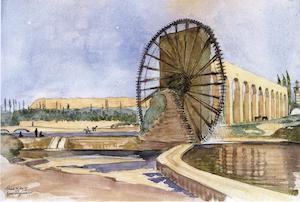
\includegraphics[width=\linewidth]{images/fugmann_water_1938.jpeg}}
        \caption{\citet{fugmann_water_1938}} 
        \label{fig:fugmann_water_1938}
    \end{subfigure}
    % \caption{Various \SEsdesigns from Ukraine and Russia documented on YouTube.}
    % \label{fig:engins:youtube}
\end{figure}


\citeauthor{samman_noria_2006}

\begin{figure}[H]
    \centering
    \begin{subfigure}{.45\textwidth}
        \centering
        \includegraphics[width=\linewidth]{images/al-dbiyat_water_2013.jpg}
        \caption{\citet{al-dbiyat_water_2013}} 
        \label{fig:al-dbiyat_water_2013}
    \end{subfigure}
    \hspace{2em}% Space between images
    \begin{subfigure}{.45\textwidth}
        \centering
        \includegraphics[width=\linewidth]{images/al-dbiyat_water_2013-1.jpg}
        \caption{\citet{al-dbiyat_water_2013}} 
        \label{fig:fugmann_water_1935-1}
    \end{subfigure}
    % \hspace{2em}% Space between images
    % \begin{subfigure}{.45\textwidth}
    %     \centering
    %     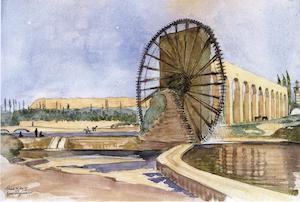
\includegraphics[width=\linewidth]{images/fugmann_water_1938.jpeg}
    %     \caption{\citet{fugmann_water_1938}} 
    %     \label{fig:fugmann_water_1938}
    % \end{subfigure}
    % \caption{Various \SEsdesigns from Ukraine and Russia documented on YouTube.}
    % \label{fig:engins:youtube}
\end{figure}


% \begin{figure}{.45\textwidth}
%     \centering
%     \includegraphics[width=\linewidth]{images/jazari_book_1974_p189.jpg}
%     \caption{\citet[p.~189, fig.~141]{jazari_book_1974}} 
%     \label{fig:jazari_book_1974}
% \end{figure}



% \begin{figure}{.45\textwidth}
%     \centering
%     \includegraphics[width=\linewidth]{images/gies_1994_chinese_wheel_p88.jpg}
%     \caption{\citet[p.~88]{giesCathedralForgeWaterwheel1994}} 
%     \label{fig:giesCathedralForgeWaterwheel1994}
% \end{figure}


NOTE: Harz Mines.

\citeauthor{monna_pb_2000}\footnote{I have relied upon GoogleTranslate for the German->English transation here.} notes that mining of Rammelsberg ore had been fully established by about 968 A.D and continued until circa 14C. However in the fourteenth century flooding and the associated diseases became a major problem in the Harz almost leading to a collapse of the industry before innovations water management systems had been implemented \citep[p.~1]{monna_pb_2000}. 

The water management systems innovations are, I contend, indicative of a new phase in the environmental research manifold. The landscape and the componentissation of the wheel as an abstract system that is not necessarily tied to the river, moreover the rivers themselvs could be controlled with a series of ponds leading to a larger scale. Over two milennia the environmental research manifold cascading transformations increasing in scale. 


\section{1564-1715 \CE: The emergence of principles in natural philosophy}
\label{sec:emerge:principle}

\begin{quotation}
    % \href{https://echo.mpiwg-berlin.mpg.de/ECHOdocuView?url=/mpiwg/online/permanent/archimedes/galil_mecha_070_en_1665&viewMode=text&pn=3&characterNormalization=regPlusNorm}{
        ``And this ought to passe for one of the benefits taken from the Mechanicks: for indeed it frequently happens, that being scanted in Force but not Time, we are put upon moving great Weights unitedly or in grosse: but he that should hope, and attempt to do the same by the help of Machines without increase of Tardity in the Moveable, would certainly be deceived, and would declare his ignorance of the use of Mechanick Instruments, and the reason of their effects.''
        % } 
        \citet[p.~3]{galilei_mechanics_1665}
\end{quotation}

In the early modern period leading up to the modern period the environmental research manifold appears to go through a further transformation. This period will be referred to as the nascent principle-based design. The argument noted above was that in the preceeding historical periods the environment had begun to be perceived, and exploited as a source of motive force. But, circa 1500-1700s, a further conceptual and perceptual development whose purpose was to solve a practical problem of \SEs power mismanagement. 

% \begin{quotation}
%     ``Firstly, for the horizontal leet, I do not consider anything else, except that, when the pipe is completely full, the water commonly leaves it twice as quickly through the hole B, as when it is only full until to F, and that the movement it has, thus leaving through this hole, carries it from BH towards E D or NC, without impeding that of its gravity, which carries it from BE towards HD. Whence it is evident that, since the water takes as much time to descend from BE to HD as it does to go from BH to NC, so that these two movements join together take it from B to C, when it is completely full, it must neither take more nor less time than before to go down from BE to HD, because it only has the same gravity; but that, during the same time, it must go twice as far from BH towards ED, because it moves twice as quickly in this sense, and since these two movements must carry it from Ba`D. 
    
%     Then, for the vertical flow, I consider, in the same way, that the force from which the water comes out of hole B causes it to rise approximately twice as fast from B to A, when the pipe is | quite full, only when it is full only up to F, and yet its gravity causes it to descend, without these two movements merging. But I consider, besides that, that its gravity does not always move it equally quickly, and that it increases by degrees the speed it gives it; so that if, for example, in one minute of time she gives it ten degrees of speed, in two minutes she must give it twenty. , and which is neither faster nor slower at the beginning than at the end, with the one whose stick PQ can be raised to R, and Firstly, for the horizontal leet, I do not consider anything else, except that, when the pipe is completely full, the water commonly leaves it twice as quickly through the hole B, as when it is only full until to F, and that the movement it has, thus leaving through this hole, carries it from BH towards E D or NC, without impeding that of its gravity, which carries it from BE towards HD. Whence it is evident that, since the water takes as much time to descend from BE to HD as it does to go from BH to NC, so that these two movements join together take it from B to C, when it is completely full, it must neither take more nor less time than before to go down from BE to HD, because it only has the same gravity; but that, during the same time, it must go twice as far from BH towards ED, because it moves twice as quickly in this sense, and since these two movements must carry it from Ba`D.

% Then, for the vertical flow, I consider, in the same way, that the force from which the water comes out of hole B causes it to rise approximately twice as fast from B to A, when the pipe is | quite full, only when it is full only up to F, and yet its gravity causes it to descend, without these two movements merging. But I consider, besides that, that its gravity does not always move it equally quickly, and that it increases by degrees the speed it gives it; so that if, for example, in one minute of time she gives it ten degrees of speed, in two minutes she must give it twenty. , and which is neither faster nor slower at the beginning than at the end, with the one whose stick PQ can be raised to R, and gravity, which however causes this drop of water to descend, from A to B, with an unequal and greater speed at the end than at the beginning, with that which one can imagine that a fourmy would have which would walk along this baston from P towards Q, at the same time as we would raise it towards R. would raise the baston, it is obvious that these two movements would cause the fourmy to remain always opposite point B; and that, if its speed is less than that of the baston, it would always rise towards 35 R; and finally that, if its speed was greater than that of the baston, it would always descend to | below B. But supposing it unequal, so that, for example, at the first step that this fourmy takes, it has only one degree of speed, at the second two, at the third three, etc., during move slower than the baston, he always raises it 40 to R, and at the point where it starts moving faster, it starts to descend, as also does each drop of water.

% Now, to guess what must be the proportion of these two movements-lie, to make the fourmy, always increasing its speed in the same way, rises only up to eight inches, while the baston will be raised slowly 45, and it rises up to three feet and 14, when it is raised twice as fast, ie use me a bit of Algebra; and I pose eight inches plus x for the line BL, at the height of which I imagine that we raise the stick PQ for one minute of time; during which minute the fourmy descends from P towards Q by the length of the line LK, which I call x, always increasing its speed; 50 so that at the end of this minute, it descends just as quickly as the baston rises, and immediately afterwards it descends more quickly. This is why it does not rise beyond the point K, which I suppose to be eight inches distant from B. After that, I reason thus: since the baston, rising slowly, has risen to the length of eight inches plus x in one minute, when it is 55 rise twice as fast, it must rise sixteen inches plus two xs for one minute, and thirty-two inches plus four xs for two minutes. And since the fourmy has taken one minute of time to acquire a speed equal to that whose stick was raised before, and that it has descended, however, by the length of the line x, it must take two minutes to acquire a 60th equal to that which it is moving now, which is double the previous one. , and during these two minutes, it must go down to the length of 4x. Because, since its speed increases in | this way, she has to travel three times as far in the second minute than in the first.

% I am,''
%     \citet[English GoogleTranslate, pp.~35-36]{verbeek_correspondence_2003}
% \end{quotation}


% \begin{figure}{.45\textwidth}
%     \centering
%     \includegraphics[width=.3\linewidth]{images/descartes_2003_verbeek_p36.jpg}
%     \caption{\citet[p.~36]{verbeek_correspondence_2003}} 
%     \label{fig:verbeek_correspondence_2003}
% \end{figure}




% \citet[p.~17]{alexanderMantraEfficiencyWaterwheel2008} argued that the issue was how to relate of the source of a water-wheel's motion to the work outcome (cause and effect). However here, I add the further 


% the wheel design 


% incentive expressed by \citeauthor{galilei_mechanics_1665} in the quote above---to reduce the economic cost of motive power---we see the rise in perception of ecological economics in its relevance to design.



% \citeauthor{davis_descartes_1986} referred to this as Torricelli's Law \citep[p.~35]{davis_descartes_1986}. 




% \begin{figure}[H]
%     \centering
%     \begin{subfigure}{.45\textwidth}
%         \centering
%         \includegraphics[width=\linewidth]{images/london_bridge_beighton_1731_p.31.jpg}
%         \caption{london_bridge_beighton_1731_p.31.jpg} 
%         \label{fig:london_bridge_beighton_1731_p}
%     \end{subfigure}
%     \hspace{2em}% Space between images
%     \begin{subfigure}{.45\textwidth}
%         \centering
%         \includegraphics[width=\linewidth]{images/London_oil_cropped.jpg}
%         \caption{London_oil_cropped} 
%         \label{fig:London_oil_cropped}
%     \end{subfigure}
%     \hspace{2em}% Space between images
%     \begin{subfigure}{.45\textwidth}
%         \centering
%         \includegraphics[width=\linewidth]{images/Machine_de_Marly.jpg}
%         \caption{Machine_de_Marly.jpg} 
%         \label{fig:Machine_de_Marly}
%     \end{subfigure}
%     \hspace{2em}% Space between images
%     \begin{subfigure}{.45\textwidth}
%         \centering
%         \includegraphics[width=\linewidth]{images/herrenhausen.jpg}
%         \caption{herrenhausen.jpg.} 
%         \label{fig:herrenhausen}
%     \end{subfigure}
%     % \caption{Various \SEsdesigns from Ukraine and Russia documented on YouTube.}
%     % \label{fig:engins:youtube}
% \end{figure}


\section{1715-1785 \CE: Principle-based design and the emergence of the maximum power principle}
\label{sec:emerge:mpp}

As shown above, the scholarship that led to \citeauthor{smeaton_experimental_1759}'s experiments is problematic since it appears to have been involved in disputes regarding the fundamental concepts of natural philosophy. In particular is the dispute well-known in the History and Philosophy of Science, between Newton and Leibniz (along with other prominent figures at that time) about \textit{vis viva} and motive force.\footnote{There is a significant amount of literature in the history and philosophy of science that is concerned with this dispute. See for example, \citet{hankins_eighteenth-century_1965, cardwell_factors_1967, iltis_controversy_1967, iltis_alembert_1970, iltis_leibniz_1971, iltis_leibnizian-newtonian_1973, gale_leibniz_1973, laudan_vis_1968-4, smith_vis_2006, hepburn_euler_2010, shimony_leibniz_2010a, reichenberger_leibnizs_2012, morris_john_2018-1}. To some extent this dispute remains unsettled with new views still emerging.}  Some disputes appear to have been about the definitions of words, intellectual property and ambiguity as much as they were about physical properties and forces.\footnote{Moreover, some of the arguments appear to have been connected with debates about perpetual motion which were prevalent at the time.} 

However \citeauthor{smeaton_experimental_1759}'s treatment appears to have generated a new concept of power, and a formalism that attempted to at one in the same time solve the \textit{vis viva} dispute but also introduce PBD. It appears to show the benefits of PBD, a benefit which had been  documented by \citeauthor{desaguliers_course_1734} in an attempt to explan of a qualitative jump in water wheel performance at the turn of the seventheenth century. 


\begin{quotation}
    ``How to measure the performance of a waterwheel remained in dispute during the eighty years spanning Smeaton's and the Franklin Institute's trials. It was a practical problem: not knowing how conceptually to relate the source of a water-wheel's motion to the work it produced made it difficult to decide where and how to construct one. Builders might have to decide whether to put a wheel on a stream with little water but a high fall or on a full stream with a low fall. They were unsure how the water acted on the wheel, not knowing whether it should go under it or over the top.'' \citet[p.~17]{alexanderMantraEfficiencyWaterwheel2008} 
\end{quotation}

\begin{quotation}
    ``Historians have described both sets of trials as attempts to measure water-wheel efficiency, and both Smeaton and the Franklin Institute did use a proto-type of efficiency, measuring the water-wheel's effect in a ratio of work done to the power, or force, used. But they did not use those words and spoke instead of “used effect,” “natural effective power,” or “mechanical power,” using terms that lacked clear and agreed-upon deffinitions. This was part of the reason for the hostility: beneath it lay the question of who had the right to define the terms.'' \citet[p.~17]{alexanderMantraEfficiencyWaterwheel2008} 
\end{quotation}

Having attempted above to show some of the emergence of the \SEs from the Ancient period, and then the rise of the concept of principle in \citeauthor*{descartes_principles_1982}' early modern natural philosophy, we now turn our attention to the experimental philosophy of \citet{smeaton_experimental_1759,smeaton_experimental_1776}'s circa 18C. 

% The analysis of \citeauthor{smeaton_experimental_1759}'s scholarship presented here diverges from that of \citeauthor{alexanderMantraEfficiencyWaterwheel2008} in two important resepcts. Firstly \citeauthor{alexanderMantraEfficiencyWaterwheel2008} uses the concept of `efficiency' as central to the analysis of \citeauthor{smeaton_experimental_1759}'s wheel. 


% Instead 
% here I emphasise \citeauthor{odum_energy_1981}'s  `energy-effectiveness'.\footnote{Odum writes, ``When we call for leaders, we speak to all, but with a different emphasis for different readers. \dots The uncommitted student may have to adopt a more realistic viewpoint and question some of his previous education regarding the rights of individuals by asking the question: Does this activity use energy effectively? That is, is it energy-effective?'' \citet[p.~2]{odum_energy_1981}} 

% ``Speed must drop and with it many of the designs that produce speed but are costly in terms of energy.'' \citet[p.~6]{odum_energy_1981}.


% This concept of \textit{effect}, as opposed to \textit{efficient}, refers back to the \textit{vis viva} controversy that \citeauthor{smeaton_experimental_1759} in part attempted to resolve thorugh his experiments on water wheels, but also wind mills.  


% Although the concept of `efficiency' (and the associated `energy-efficiency') is an important one grounding much of \citeauthor{alexanderMantraEfficiencyWaterwheel2008}'s narrative regarding the history and philosophy of mechanical engineering, 



% What Odum called the `force-flux law'---expressed by the relations \(J = CX, or X = JR\)---which is what Galileo and Toritelli both addressed. However in the view of.  



% If they could not understand the force-flux law, then it, ``\dots made it difficult to decide where and how to construct one.'' \citet[p.~17]{alexanderMantraEfficiencyWaterwheel2008}.



% \citeauthor{morris_john_2018-1} 

% Engineer and historian Walter Vincenti has argued that \citeauthor{smeaton_experimental_1759}

% parameter variation





% power, power maximisation and

% This section seeks to show the rise of both principle- of how 

% \citet[p.~17]{alexanderMantraEfficiencyWaterwheel2008} 

% It was a practical problem: not knowing how conceptually to relate the source of a water-wheel's motion to the work it produced made it difficult to decide where and how to construct one.


% As both Vincenti and \citeauthor{channell_emergence_2019} have argued, 





% method of experiments involved what is now called “parameter variation,” in which one parameter, such as the head, or quantity of water, or speed, is varied while the other parameters are held constant. Vincenti has demonstrated that this experimental methodology became a fundamental aspect of modern engi- neering science (Vincenti 1990, pp. 146–151).




% In the period after \citeauthor{smeaton_experimental_1776}'s \citeyear{smeaton_experimental_1776} article on mechanic power, 

\section{1860-1912 \CE: Specialisation then Generalisation }
\label{sec:reemerge:mpp}

% In the period following \citeauthor{smeaton_experimental_1776}'s \citeyear{smeaton_experimental_1776} article on mechanic power, the concepts associated with steam, electro magnetism and atomic energy were among some of the major technologies that ushered in the industrial revolution. It appears that this was a period of intellectual specialization where the focus was on the derivation of theorems and principles relevant to specific domains.  



% \section{The emergence of maximum power as a general principle for system design}
% \label{chp:mpp:gest}

% % \subsection{The emergence of power and principle in design}
% % \label{sec:emergence}

% It then appears to have been recognised separately as a theorem in different domains with no analogical transfers until \citeauthor{lotka_law_1945} proposed it as a general principle for evolutionary systems. The subsequent effort by the EGST paradigm was to build transdisciplinary methods for analogical transfer, so that the \mpps could be identified and used as a design aid in different disciplines.



% The main contention here is that 


% This chapter then seeks to look at the literature of these three periods to answer the following questions: What is the \SE? What is the \mpp? What is a principle? Was the performance jump in \textit{Stesibuque Engins} due to the introduction of principle-based design, and a recognition of the significance of \mpps for design?

% and 
% selection criterion for sustainable designs and may explain the subsequent jump in water wheel per

% there it was the recognition of the \mpp as a design principle which enabled the jump in pumping water wheel performance in the early modern period. 

% However, to motivate this review the chapter will start with contemporary quantitative, model-based sustainability theory which has arisen from ecosystems scholarship. 

% \include{principles.tex}

\chapter{Lit. Rev. Part B }
\label{part:b}

% \section{\textit{A sine theoria cum doctrina}  }

% \section{Contemporary examples from around the world}

% With the aid of the YouTube suggestions algorithm, I have been able to collate screenshots contemporary examples of the \SEsspread throughout the world. 

% What I hope to illustrate through these examples is that it is quite difficult to ascertain whether or not any of the wheels show evidence of principle-based design. By the end of this thesis, it is hoped that we may be able to determine this either by eye, or by estimations. 

% The selection documented below appears to show a chaotic design practice. None of the two wheels are alike. Here we are not looking at the materials for the likeness, but rather the circumference of wheel, the size of bucket, the number of buckets, and the size and number of paddles. For, as noted in the pre-history given in Part I, these are the key parameters for our analysis. 

% Have all of the wheels naturally embodied the principle-based design, or are some of them simply random designs?

% \subsection{Examples from China}

% elainehuang_ancient_2020


% \begin{figure}[H]
%     \centering
%     \begin{subfigure}{.45\textwidth}
%         \centering
%         \includegraphics[width=\linewidth]{images/wildenburg_china_2010.jpg}
%         \caption{\citet{wildenburg_china_2010}.}  
%         \label{fig:wildenburg}
%     \end{subfigure}
%     \hspace{2em}% Space between images
%     \begin{subfigure}{.45\textwidth}
%         \centering
%         \includegraphics[width=\linewidth]{images/zukeikomiya_shangkara_2012.jpg}
%         \caption{Screenshot of video by YouTube user \citet{zukeikomiya_shangkara_2012}.}
%         \label{fig:zukeikomiya}
%     \end{subfigure}%
%     \hspace{2em}% Space between images
%     \begin{subfigure}{.45\textwidth}
%         \centering
%         \includegraphics[width=\linewidth]{images/minami365_zizuonoshuichedesu_2012.jpg}
%         \caption{Screenshot of video by YouTube user \citet{minami365_zizuonoshuichedesu_2012}.} 
%         \label{fig:minami365}
%     \end{subfigure}
%     \hspace{2em}% Space between images
%     \begin{subfigure}{.45\textwidth}
%         \centering
%         \includegraphics[width=\linewidth]{images/kazumarutv_nodokanatianyuanfengjing_2013.jpg}
%         \caption{Screenshot of video by YouTube user \citet{kazumarutv_nodokanatianyuanfengjing_2013}.}  
%         \label{fig:kazumarutv}
%     \end{subfigure}

    

%     \caption{Various \SEsdesigns documented on YouTube.}
%     \label{fig:engins:youtube}
% \end{figure}

% \subsection{Examples from Japan}

% \begin{figure}[H]
%     \centering
%     \begin{subfigure}{.45\textwidth}
%         \centering
%         \includegraphics[width=\linewidth]{images/turunasi_tiannbonishuiwoyinkushuiche_2014.jpg}
%         \caption{}\label{fig:turunasi}
%     \end{subfigure}
%     \hspace{2em}% Space between images
%     \begin{subfigure}{.45\textwidth}
%         \centering
%         \includegraphics[width=\linewidth]{images/minouscape_shengmarebianwatutalingyenosanlianshuiche_2015.jpg}
%         \caption{}\label{fig:minouscape}
%     \end{subfigure}
%     \hspace{2em}% Space between images
%     \begin{subfigure}{.45\textwidth}
%         \centering
%         \includegraphics[width=\linewidth]{images/bideoxingjiao_zhaocangsanlianshuicheshidong2009_2009.jpg}
%         \caption{}\label{fig:bideoxingjiao}
%     \end{subfigure}
%     \hspace{2em}% Space between images
%     \begin{subfigure}{.45\textwidth}
%         \centering
%         \includegraphics[width=\linewidth]{images/3bonjp_niukeshouyongshui_2012.jpg}
%         \caption{}\label{fig:3bonjp}
%     \end{subfigure}
%     \hspace{2em}% Space between images
%     \begin{subfigure}{.45\textwidth}
%         \centering
%         \includegraphics[width=\linewidth]{images/hkawa_4k_2020.jpg}
%         \caption{}\label{fig:hkawa}
%     \end{subfigure}
%     \caption{\ref{fig:turunasi} \citet{turunasi_tiannbonishuiwoyinkushuiche_2014}, \ref{fig:minouscape} \citet{minouscape_shengmarebianwatutalingyenosanlianshuiche_2015}, \ref{fig:bideoxingjiao} \citet{bideoxingjiao_zhaocangsanlianshuicheshidong2009_2009} (Also see \citet{asakura_asakura_2020}), \ref{fig:3bonjp} \citet{3bonjp_niukeshouyongshui_2012},  \ref{fig:hkawa} \citet{hkawa_4k_2020}, }
%     \label{fig:engins:japan}
% \end{figure}





% \subsection{Examples from Syria}

% \begin{figure}[H]
%     \centering
%     \begin{subfigure}{.45\textwidth}
%         \centering
%         \includegraphics[width=\linewidth]{images/yaseryusuf_siria_2009.jpg}
%         \caption{}\label{fig:yaseryusuf}
%     \end{subfigure}
%     \begin{subfigure}{.45\textwidth}
%         \centering
%         \includegraphics[width=\linewidth]{images/paulharvey_hama_2010.jpg}
%         \caption{}\label{fig:epsos}
%     \end{subfigure}
%     \caption{\ref{fig:yaseryusuf} \citet{yaseryusuf_siria_2009}, \ref{fig:epsos} \citet{paulharvey_hama_2010}}
%     \label{fig:engins:youtube}
% \end{figure}

% \subsection{Examples from Germany}

% \begin{figure}[H]
%     \centering
%     \begin{subfigure}{.45\textwidth}
%         \centering
%         \includegraphics[width=\linewidth]{images/epsos.de_wooden_2015.jpg}
%         \caption{}\label{fig:epsos}
%     \end{subfigure}
%     \caption{\ref{fig:epsos} \citet{epsos.de_wooden_2015},}
%     \label{fig:engins:youtube}
% \end{figure}


% \subsection{Examples from Ukraine and Russia}

% \begin{figure}[H]
%     \centering
%     \begin{subfigure}{.45\textwidth}
%         \centering
%         \includegraphics[width=\linewidth]{images/3jlou_4utep_vodyane_2016.jpg}
%         \caption{Screenshot of video by a Ukrainian YouTube user \citet{3jlou_4utep_vodyane_2016}.} 
%         \label{fig:3jlou_4utep}
%     \end{subfigure}
%     \caption{Various \SEsdesigns from Ukraine and Russia documented on YouTube.}
%     \label{fig:engins:youtube}
% \end{figure}


% \subsection{Examples from Persia}

% \begin{figure}[H]
%     \centering
%     \begin{subfigure}{.45\textwidth}
%         \centering
%         \includegraphics[width=\linewidth]{images/asiffarid_water_2012.jpg}
%         \caption{\citet{asiffarid_water_2012}.} 
%         \label{fig:3jlou_4utep}
%     \end{subfigure}
%     % \caption{Various \SEsdesigns from Ukraine and Russia documented on YouTube.}
%     % \label{fig:engins:youtube}
% \end{figure}


% \subsection{Examples from Indonesia}

% \begin{figure}[H]
%     \centering
%     \begin{subfigure}{.45\textwidth}
%         \centering
%         \includegraphics[width=\linewidth]{images/muhammadfaridrizqi_pengairan_2020.jpg}
%         \caption{}\label{fig:rizqi}
%     \end{subfigure}
%     \hspace{2em}% Space between images
%     \begin{subfigure}{.45\textwidth}
%         \centering
%         \includegraphics[width=\linewidth]{images/rhmtdns_berkas_2021.jpg}
%         \caption{}\label{fig:rhmtdns}
%     \end{subfigure}
%     \caption{\ref{fig:rizqi} \citet{rizqi_pengairan_2020},\ref{fig:rhmtdns}} \citet{rhmtdns_berkas_2021}}
%     \label{fig:engins:youtube}
% \end{figure}



% \subsection{Examples from Vietnam}

% \begin{figure}[H]
%     \centering
%     \begin{subfigure}{.45\textwidth}
%         \centering
%         \includegraphics[width=\linewidth]{images/angelpham_water_2017.jpg}
%         \caption{}\label{fig:angelpham}
%     \end{subfigure}
%     \hspace{2em}% Space between images
%     % \begin{subfigure}{.45\textwidth}
%     %     \centering
%     %     \includegraphics[width=\linewidth]{images/rhmtdns_berkas_2021.jpg}
%     %     \caption{}\label{fig:rhmtdns}
%     % \end{subfigure}
%     \caption{\ref{fig:angelpham} \citet{angelpham_water_2017}}
%     \label{fig:engins:youtube}
% \end{figure}




% \section{ Electric Analogs and Self-organisation with out \mpp}

% ``The art object is replaced by participation in the art process. This is the essential meaning of electric circuitry and responsive environments. The artist leaves the Ivory Tower for the Control Tower, and abandons the shaping of art objects in order to program the environment itself as a work of art.'' \citet[p.~xv, citing McLuhan]{busbea_responsive_2019}


% \section{Parametric Schematics - The path is not the path}

% \include{parametric_problem.tex}

% \section{Introduction to General Ecological Systems Theory (GEST)}

% evolutionary domestic eco-systems, responsive environments, a new peace and joy.”


% \section{GEST and issues in contemporary sustainability theory}
% \label{sec:gest}


% An issue facing contemporary sustainability theory is that it does not appear to be a unified field with an agreed methodology. Whilst some sustainability literature is quantitative and uses quantitative models to simulate systems, other sustainability literature does not, preferring qualitative means and mediums of communication. A scientific method that is itself concerned with hypothesis testing can use the tools of quantification, mathematical modelling and simulation as cornerstones in enabling repeatable and verifiable claims about sustainability. Epistemologically speaking, repeatability and verifiability are important factors when seeking to develop a scientific view of sustainability. Non-quantitative communication about sustainability may not seek a scientific epistemology or way of knowing. With such an epistemic divide it is difficult to know how to proceed.  

% Perhaps as an attempt to bridge the quantitative/non-quantitative divide, beginning with H.T.Odum and colleagues systems ecologists introduced qualitative network diagrams and schematics as a means of introducing non-quantitative scholarship to quantitative procedures. H.T.Odum's scholarship has been considered pivotal to the establishment of quantitative ecology and the concept of the `ecosystem' together with the quantitative analysis of ecosystem sustainability. Just before Odum's death, \citeauthor{odum_modeling_2000} attempted to show how the assignment of numerical values to network diagrams could be used to represent concepts and summarise data together with the ability to calibrate simulation equations \citep[p.~40]{odum_modeling_2000}. In Chapter 3  of their book \textit{Modeling for All Scales}, \citeauthor{odum_modeling_2000} attempted to explain the, ``\dots different ways to use numbers on energy systems diagrams consistent with principles for energy and matter processing'' \citep[p.~40]{odum_modeling_2000}.

% This thesis attempts to follow the \citeauthor{odum_modeling_2000}'s approach, however in doing so further counterintuitive concepts and non-standard terminology are required to comprehend their paradigm sufficiently.  The first concept is that of the ``principles for energy and matter processing'' mentioned by \citeauthor{odum_modeling_2000} in the quote above. One of the principles is what has eventually become known as the  Maximum Power Principle (\mpp) which has been talked about as an evolutionary principle of self-organization.Other words that have been created by the Odum school are things like, `\textbf{emergy}' \citep{scienceman_energy_1987, odum_emergy_1991, odum_emergy_1995, odum_environmental_1995,  le_corre_emergy_2016}, `\textbf{empower}' \citep{beni_maximum_2012} and `\textbf{transformity}' each apparently with specific and quantifiable meaning, but themselves not well-defined. 

% Of this movement, in \citeyear{braham_environmental_2013} \citeauthor{braham_environmental_2013} questioned 
% self-organization for maximum power could offer any criteria for environmental building design, and concluded that the approach of introducing ecological hierarchy to the expression of power, ``\dots opens the topic of sustainable design to its proper scope \dots'' \citep[p.~141]{braham_environmental_2013}. However \citeauthor{moe_energy_2017} has rallied against the,  ``\dots epistemological and methodological damage wrought by the autarky of sustainability and the autonomy of formal discourse'', and argued that, ``\dots architects now need both fresh technical methodologies and evolved design methodologies for design with respect to energy and matter'' \citep[p.~8]{moe_energy_2017}. 


% \subsection{The ecological and general systems paradigm}
% \label{sec:egs}





% Models with autocatalytic feedbacks utilized more power than the same models with only linear pathways.


% tested different configurations by either varying resource availability or keeping it constant to establish whether a modelled systems could maximize power as the criterion for utility and success.


% In contract the present thesis is concerned with the geometric principles and mechanics that can be used as a design aid of autocatalytic systems.   






% \include{gest.tex}



% \subsection{Identifying the GEST challenge for ESD Parametric Design}

% \include{gest_challenge_to_pd.tex}

% Biliography


\addcontentsline{toc}{section}{References}
\bibliography{MyLibrary}
\printbibliography



\end{document}